%%%%%%%%%%%%%%%%%%%%%%%%%%%%%%%%%%%%%%%%%%  不使用 authblk 包制作标题  %%%%%%%%%%%%%%%%%%%%%%%%%%%%%%%%%%%%%%%%%%%%%%
%-------------------------------PPT Title-------------------------------------
\title{$10^3$原子量级模型高精度第一原理计算实现}
%-----------------------------------------------------------------------------

%----------------------------Author & Date------------------------------------
\author[]{\vskip +10pt 李计勇、李珅; 崔旭、姜骏\inst{}} %[]{} (optional, use only with lots of authors)
%% - Give the names in the same order as the appear in the paper.
%% - Use the \inst{?} command only if the authors have different
%%   affiliation.
\institute[BCC]{\inst{}%
%\institute[Gain~Strong]{\inst{}%
\vskip -15pt 南京展智科技有限公司\\北京市计算中心~材料计算团队}
%\vskip -20pt {\large 格致斯创~科技}}
\date[\today] % (optional, should be abbreviation of conference name)
{	%{\fontsize{6.2pt}{4.2pt}\selectfont{\textcolor{blue}{E-mail:~}\url{jiangjun@bcc.ac.cn}}}
\vskip 45 pt {\fontsize{8.2pt}{6.2pt}\selectfont{%清华大学\;\;物理系% 报告地点
	\vskip 5 pt \textrm{2025.09.04}}}
}

%% - Either use conference name or its abbreviation
%% - Not really information to the audience, more for people (including
%%   yourself) who are reading the slides onlin%%   yourself) who are reading the slides onlin%%   yourself) who are reading the slides onlineee
%%%%%%%%%%%%%%%%%%%%%%%%%%%%%%%%%%%%%%%%%%%%%%%%%%%%%%%%%%%%%%%%%%%%%%%%%%%%%%%%%%%%%%%%%%%%%%%%%%%%%%%%%%%%%%%%%%%%%

\subject{}
% This is only inserted into the PDF information catalog. Can be left
% out.
%\maketitle
\frame
{
%	\frametitle{\fontsize{9.5pt}{5.2pt}\selectfont{\textcolor{orange}{“高通量并发式材料计算算法与软件”年度检查}}}
\titlepage
}
%-----------------------------------------------------------------------------

%------------------------------------------------------------------------------列出全文 outline ---------------------------------------------------------------------------------
\section*{}
\frame[allowframebreaks]
{
	\frametitle{\textrm{Outline}}
%  \frametitle{\textcolor{mycolor}{\secname}}
  \tableofcontents%[current,currentsection,currentsubsection]
}
%在每个section之前列出全部Outline
%类似的在每个subsection之前列出全部Outline是\AtBeginSubsection[]
%\AtBeginSection[]
%{
%  \frame<handout:0>%[allowframebreaks]
%  {
%    \frametitle{Outline}
%%全部Outline中,本部分加亮
%    \tableofcontents[current,currentsection]
%  }
%}

%-----------------------------------------------PPT main Body------------------------------------------------------------------------------------
\small
\section{研究背景}
\begin{frame}
	\frametitle{千原子量级模型计算的必要性和困难}
	材料的属性由其基本组分、结构决定:
%			\\材料功能与性质的精确描述,必须考察材料的复杂性
\begin{figure}[h!]
\vspace*{-0.10in}
%\centering
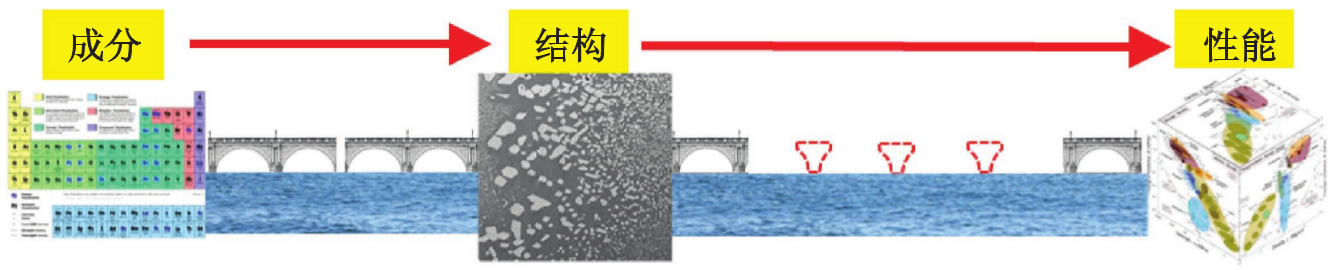
\includegraphics[height=0.80in,width=4.05in]{Figures/MGE-2.png}
%\caption{\tiny \textrm{Pseudopotential for metallic sodium, based on the empty core model and screened by the Thomas-Fermi dielectric function.}}%(与文献\cite{EPJB33-47_2003}图1对比)
%\vskip 0.05pt
%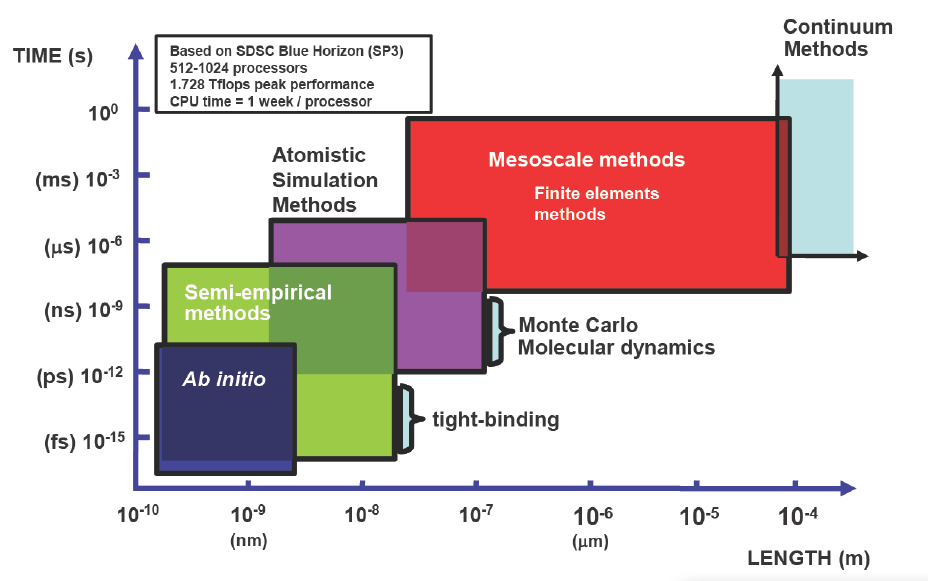
\includegraphics[height=2.20in,width=3.45in]{Figures/Multi-Scale-6.png}
%\caption{\tiny \textrm{Pseudopotential for metallic sodium, based on the empty core model and screened by the Thomas-Fermi dielectric function.}}%(与文献\cite{EPJB33-47_2003}图1对比)
\label{Multi-Scale-1}
\end{figure}
% 调节材料的组分获得材料的特性:~掺杂、表面等特性
	材料模拟与计算在新材料研发中的作用日益凸显
	\begin{itemize}
		\item \textcolor{blue}{功能材料}的属性精确调控:\\
			对材料组分与结构存在客观要求
		\item \textcolor{blue}{结构材料}的微观缺陷和应力研究:\\
			对材料尺度也有客观要求
		\item \textrm{AI}支持的\textcolor{blue}{跨尺度材料模拟}:\\
			对模型和数据同样有尺度要求
	\end{itemize}
\end{frame}

\begin{frame}
	\frametitle{千原子量级模型计算的必要性和困难}
	第一原理计算(主要是\textrm{DFT})为材料模拟提供``数据底座'':
%			\\为包括微观电子结构性质在内的基本物性提供有效描述
\begin{figure}[h!]
\vspace*{-0.10in}
%\centering
%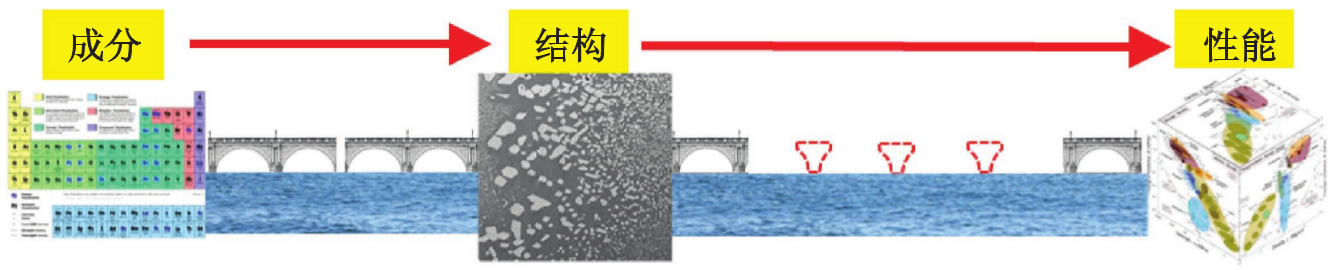
\includegraphics[height=0.60in,width=3.05in]{Figures/MGE-2.png}
%\caption{\tiny \textrm{Pseudopotential for metallic sodium, based on the empty core model and screened by the Thomas-Fermi dielectric function.}}%(与文献\cite{EPJB33-47_2003}图1对比)
%\vskip 0.05pt
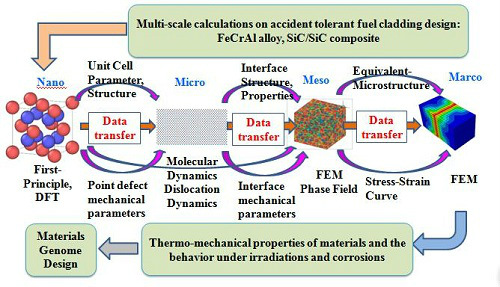
\includegraphics[height=2.50in,width=4.05in]{Figures/Multi_Scale-5.jpg}
%\caption{\tiny \textrm{Pseudopotential for metallic sodium, based on the empty core model and screened by the Thomas-Fermi dielectric function.}}%(与文献\cite{EPJB33-47_2003}图1对比)
\label{Multi-Scale-2}
\end{figure}
\end{frame}

\begin{frame}
	\frametitle{千原子量级模型计算的必要性和困难}
	\textrm{DFT}可以精确模拟的材料尺度非常有限:
\begin{figure}[h!]
%\vspace*{-0.10in}
%\centering
%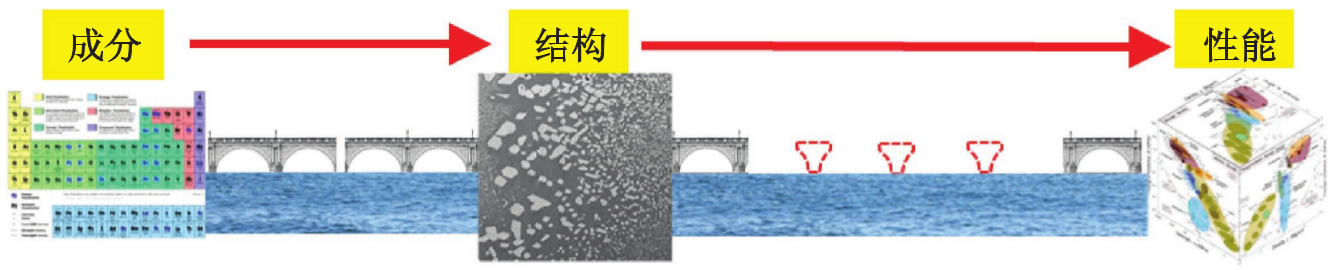
\includegraphics[height=0.60in,width=3.05in]{Figures/MGE-2.png}
%\caption{\tiny \textrm{Pseudopotential for metallic sodium, based on the empty core model and screened by the Thomas-Fermi dielectric function.}}%(与文献\cite{EPJB33-47_2003}图1对比)
%\vskip 0.05pt
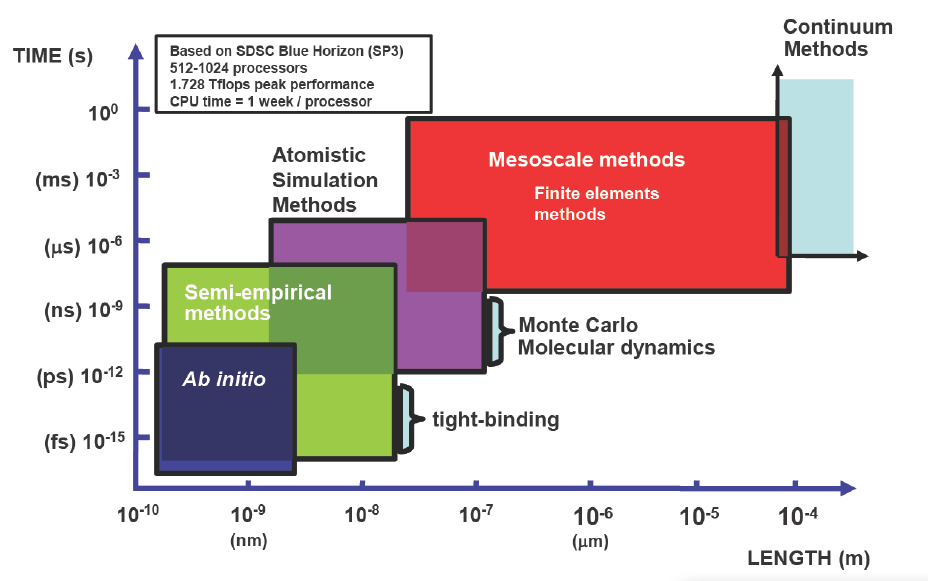
\includegraphics[height=2.50in,width=4.00in]{Figures/Multi-Scale-6.png}
%\caption{\tiny \textrm{Pseudopotential for metallic sodium, based on the empty core model and screened by the Thomas-Fermi dielectric function.}}%(与文献\cite{EPJB33-47_2003}图1对比)
\label{Multi-Scale-3}
\end{figure}
\end{frame}

\begin{frame}
	\frametitle{千原子量级模型计算的必要性和困难}
	\begin{itemize}
		\item 机器学习势函数,要考虑粒子间多体相互作用与长程相互作用
\begin{figure}[h!]
\vspace*{-0.10in}
%\centering
%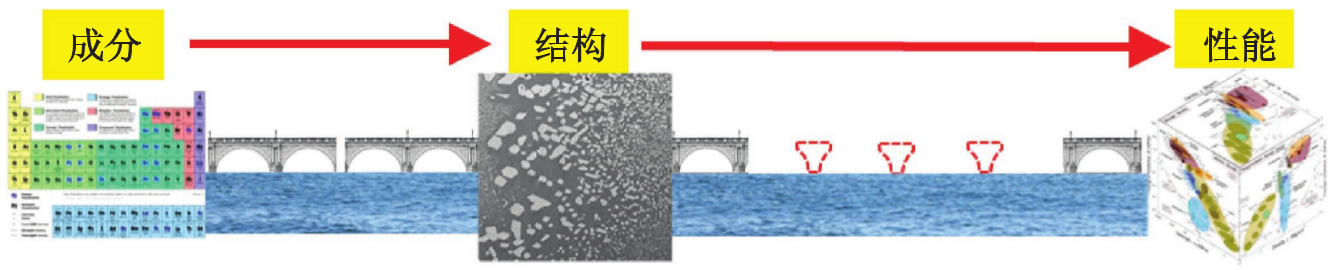
\includegraphics[height=0.60in,width=3.05in]{Figures/MGE-2.png}
%\caption{\tiny \textrm{Pseudopotential for metallic sodium, based on the empty core model and screened by the Thomas-Fermi dielectric function.}}%(与文献\cite{EPJB33-47_2003}图1对比)
%\vskip 0.05pt
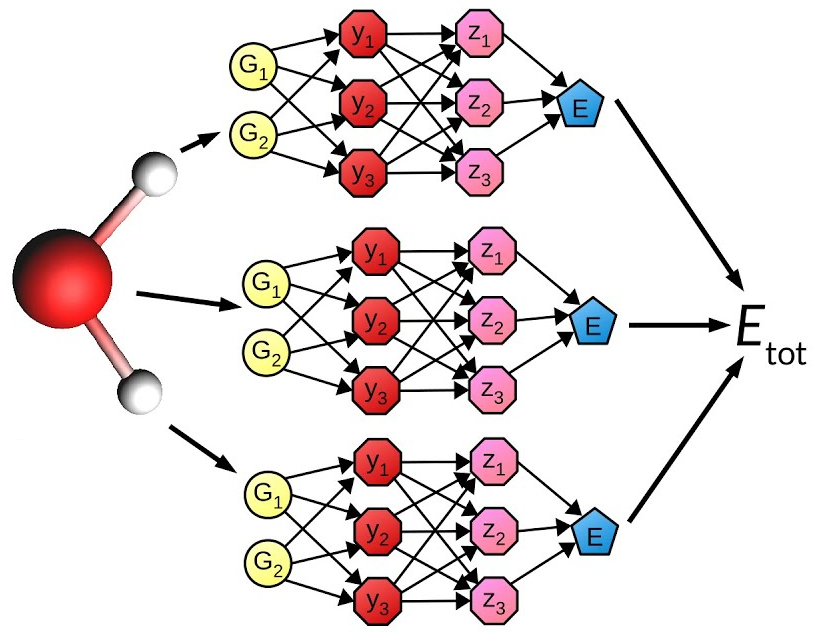
\includegraphics[height=2.34in,width=3.00in]{Figures/MLP_GNN.jpg}
%\caption{\tiny \textrm{Pseudopotential for metallic sodium, based on the empty core model and screened by the Thomas-Fermi dielectric function.}}%(与文献\cite{EPJB33-47_2003}图1对比)
\label{Multi-Scale-4}
\end{figure}
	\end{itemize}
\end{frame}

\section{\rm{VASP}软件的主要瓶颈}
\frame
{
	\frametitle{\textrm{VASP}软件简介}
	\textrm{VASP}软件是维也纳大学\textrm{(Universit\"at Wien)}~\textrm{G. Kresse}等开发的第一原理模拟软件包,在物理方法、优化算法和并行计算实现等方面都有出色的性能,是第一原理计算软件中``执牛耳''者
	\begin{itemize}
\fontsize{7.2pt}{5.2pt}\selectfont
		\item \textrm{VASP}采用\textrm{PAW~(Projector Augmented-Wave)}方法,平衡了赝势方法和全电子计算优点,兼顾了计算的精度和效率
		\item \textrm{VASP}在实空间优化投影函数\textrm{(Projector)},将主要的计算过程变换到实空间完成,节省了矩阵迭代的内存开销%,保证了计算精度和效率
		\item \textrm{VASP}通过引入多样的优化算法,提高了矩阵对角化和电荷密度搜索的效率
		\item 在\textrm{VASP}的并行计算中,有效均衡了各节点处理\textrm{FFT}变换负载和通信,提升了软件的并行效率
	\end{itemize}
\begin{figure}[h!]
	\vspace{-0.25in}
\centering
%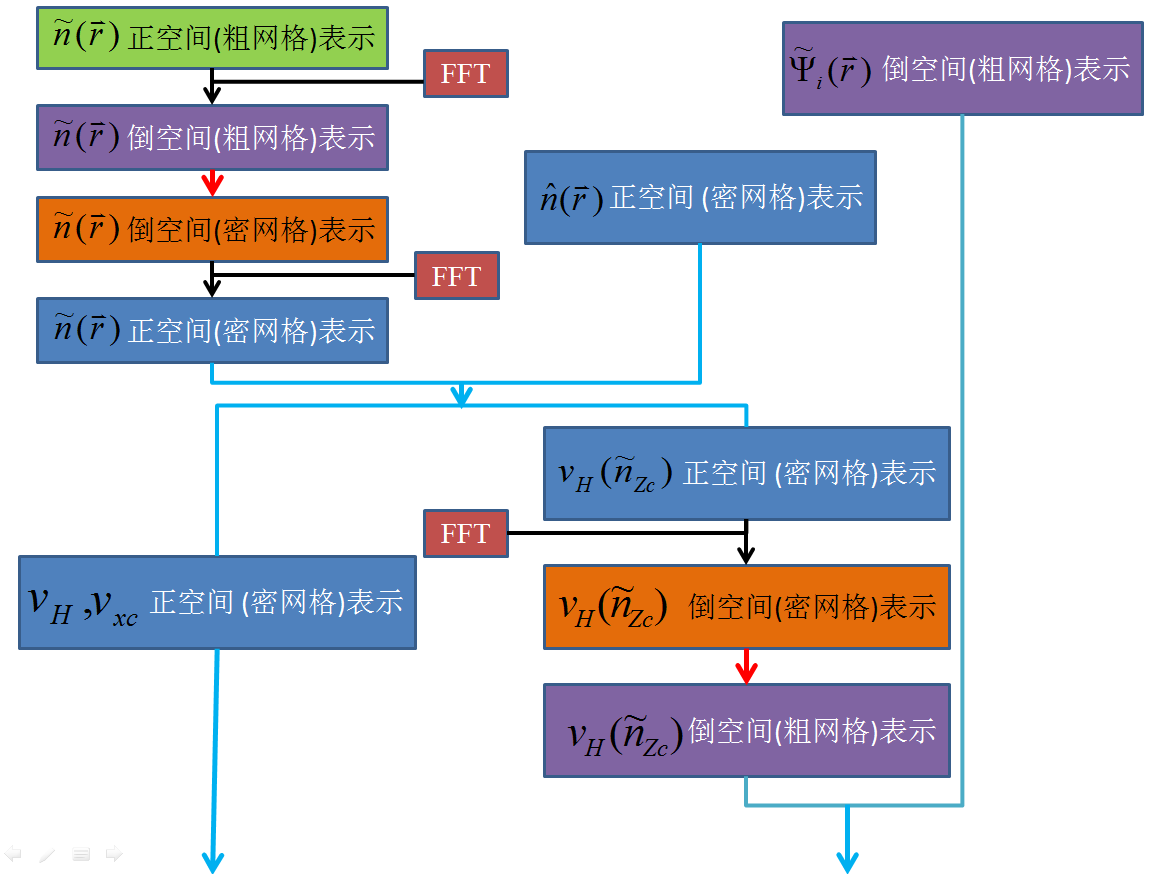
\includegraphics[height=2.7in,width=4.0in,viewport=0 0 1180 875,clip]{Figures/dual_grid.png}
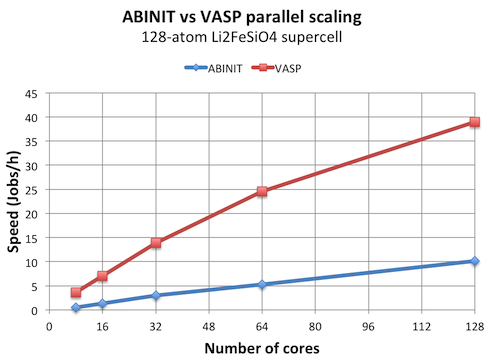
\includegraphics[height=1.55in,width=2.05in,viewport=0 0 240 200,clip]{Figures/VASP-abinit_Li128-2.png}
%\caption{\tiny \textrm{The comparison of parallel scaling for ABINIT vs VASP.}}%(与文献\cite{EPJB33-47_2003}图1对比)
\label{ABINIT_vs_VASP-1}
\end{figure} 
}

%\frame
%{
%	\frametitle{\textrm{VASP}的开发团队}
%\begin{figure}[h!]
%\centering
%\vspace*{-0.25in}
%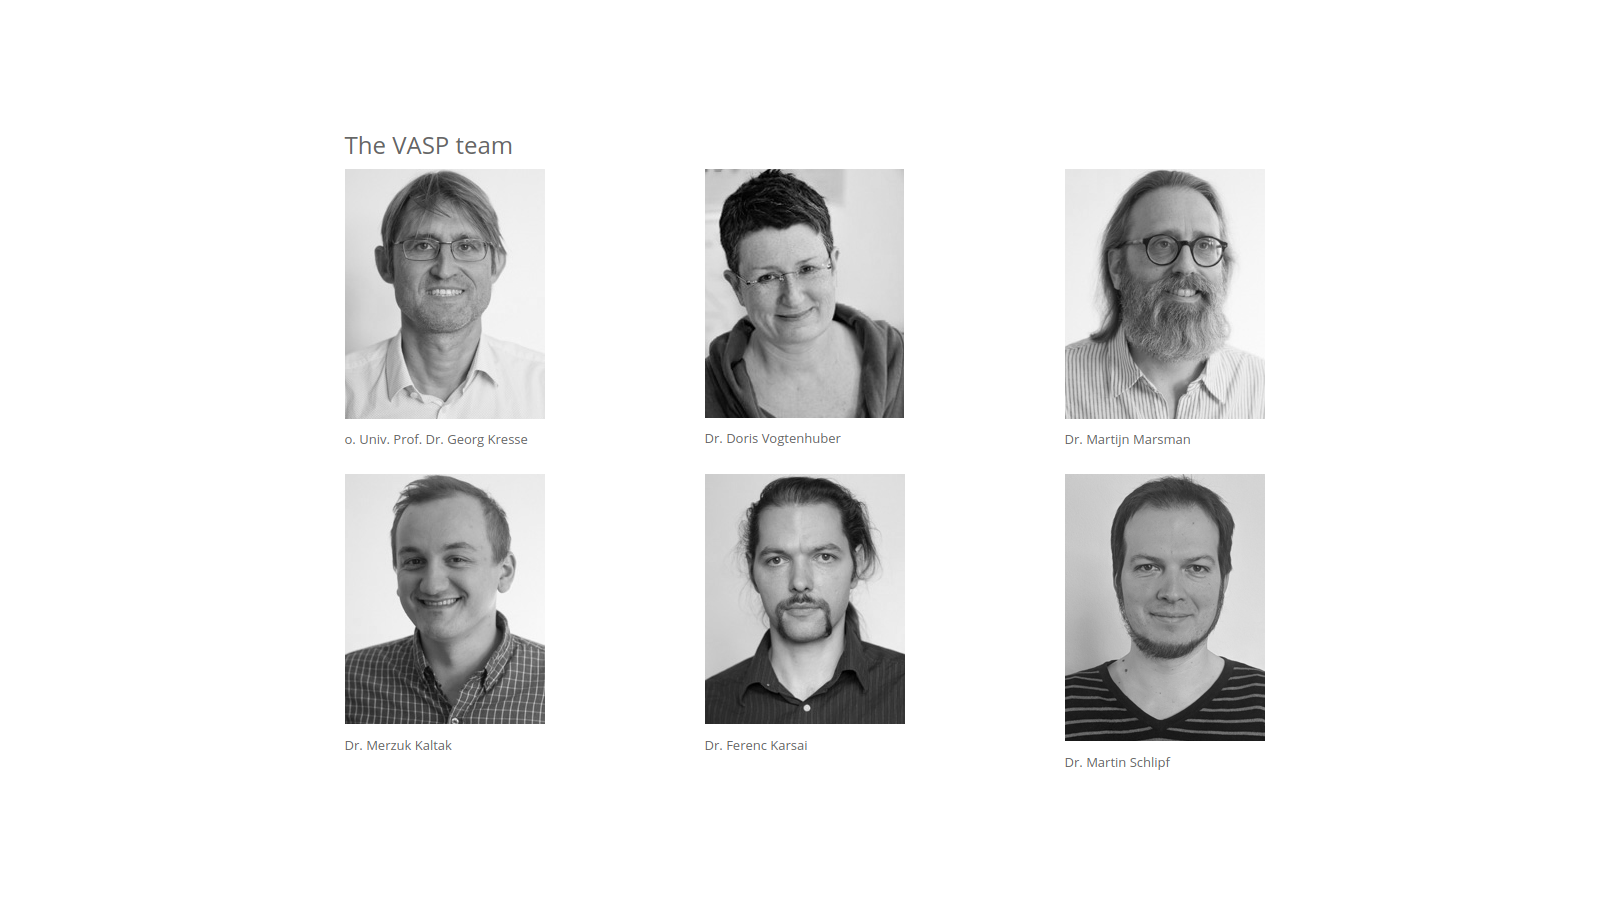
\includegraphics[height=2.70in,width=4.05in,viewport=330 130 1280 770,clip]{Figures/VASP_team.png}
%\caption{\tiny \textrm{The development team of VASP.}}%(与文献\cite{EPJB33-47_2003}图1对比)
%\label{VASP_team}
%\end{figure}
%}
%
%\frame
%{
%	\frametitle{\textrm{VASP}的\textrm{Kohn-Sham}方程求解流程}
%\begin{figure}[h!]
%	\vspace{-0.2in}
%\centering
%%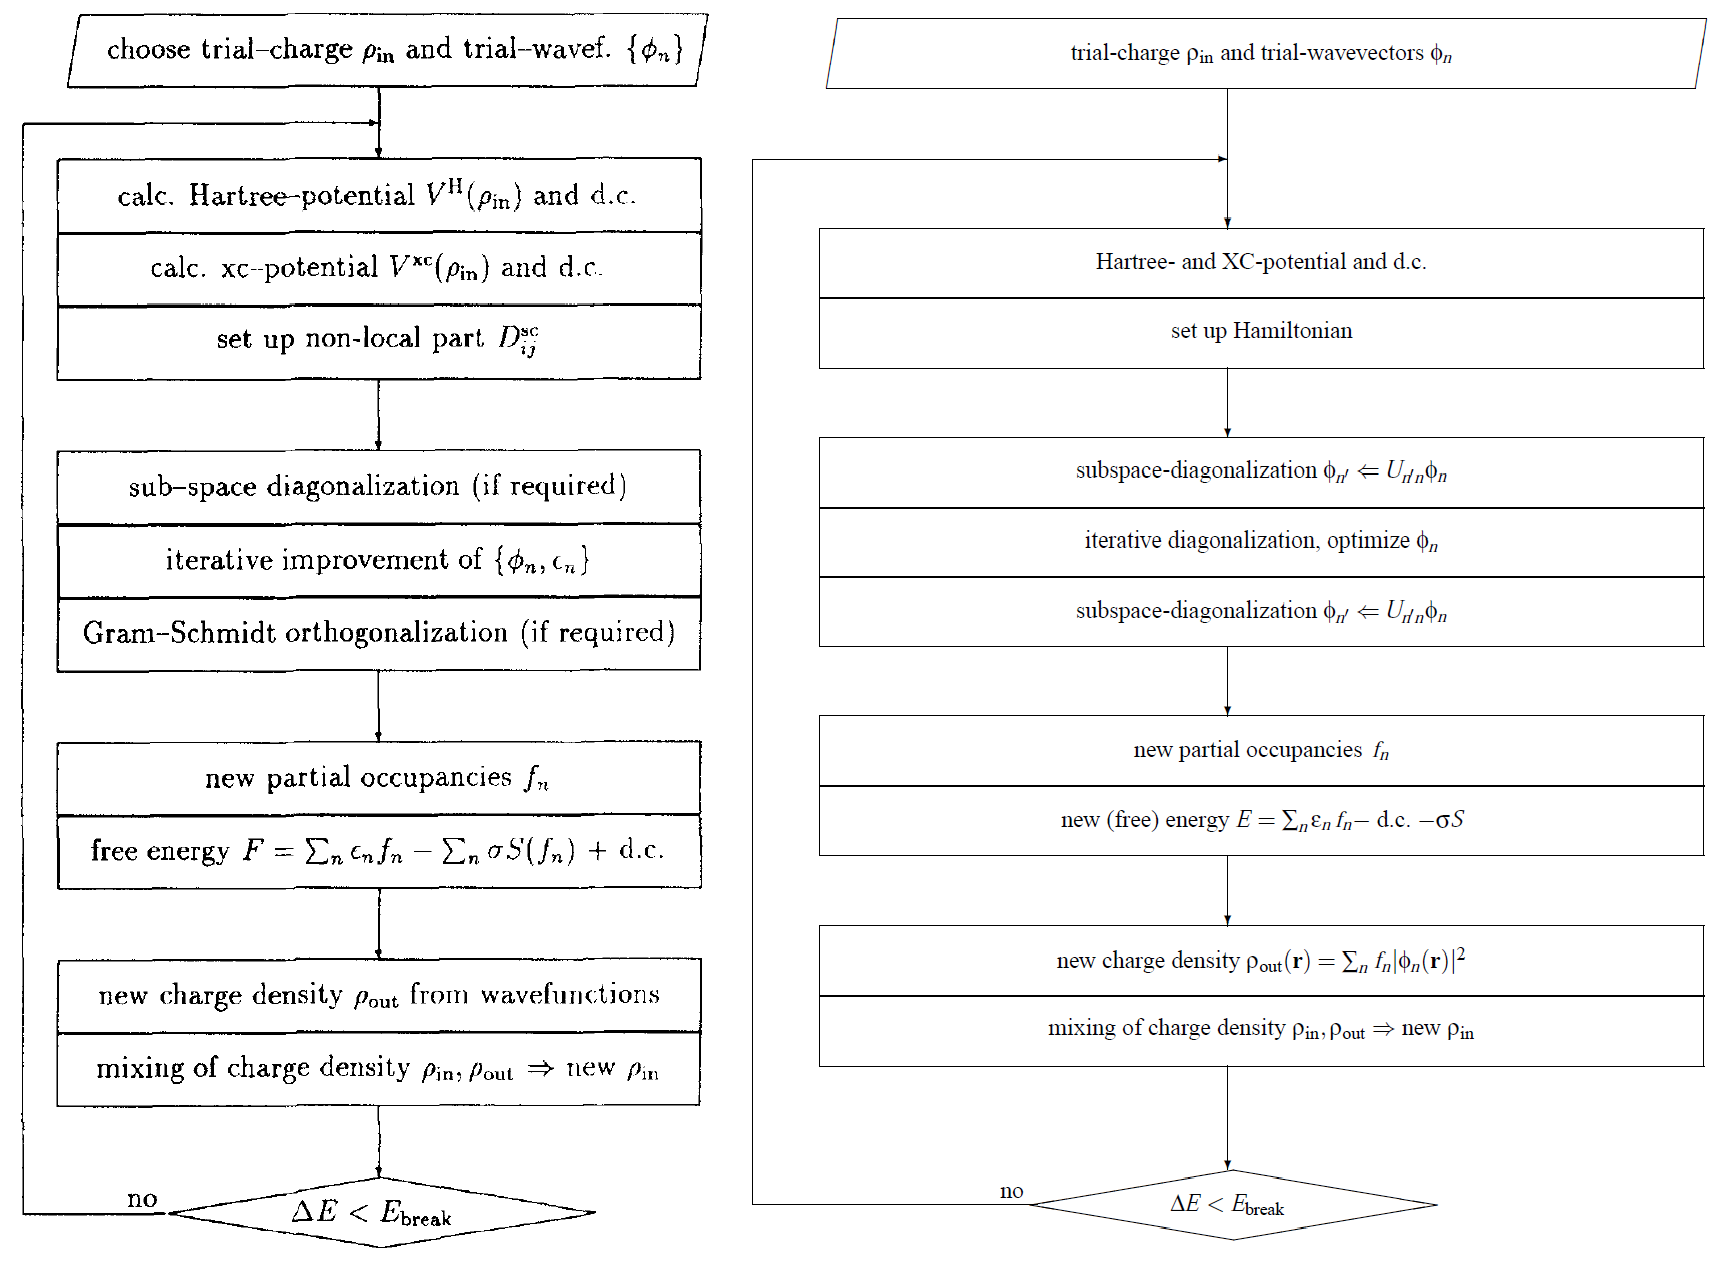
\includegraphics[height=2.7in,width=4.0in,viewport=0 0 1300 960,clip]{Figures/VASP_procedure-full.png}
%%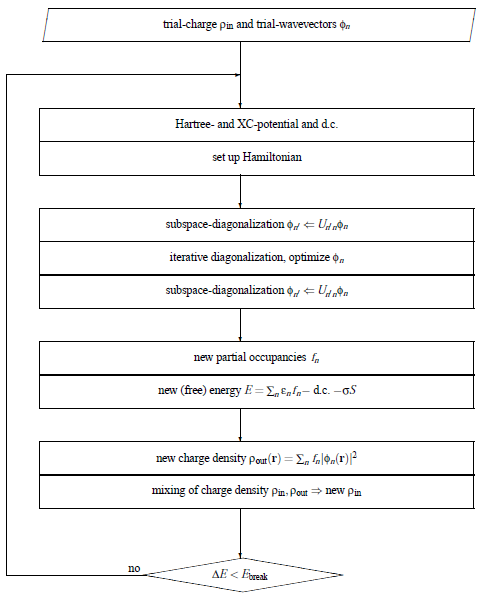
\includegraphics[height=2.1in,width=1.6in,viewport=0 0 480 630,clip]{Figures/VASP_procedure.png}
%%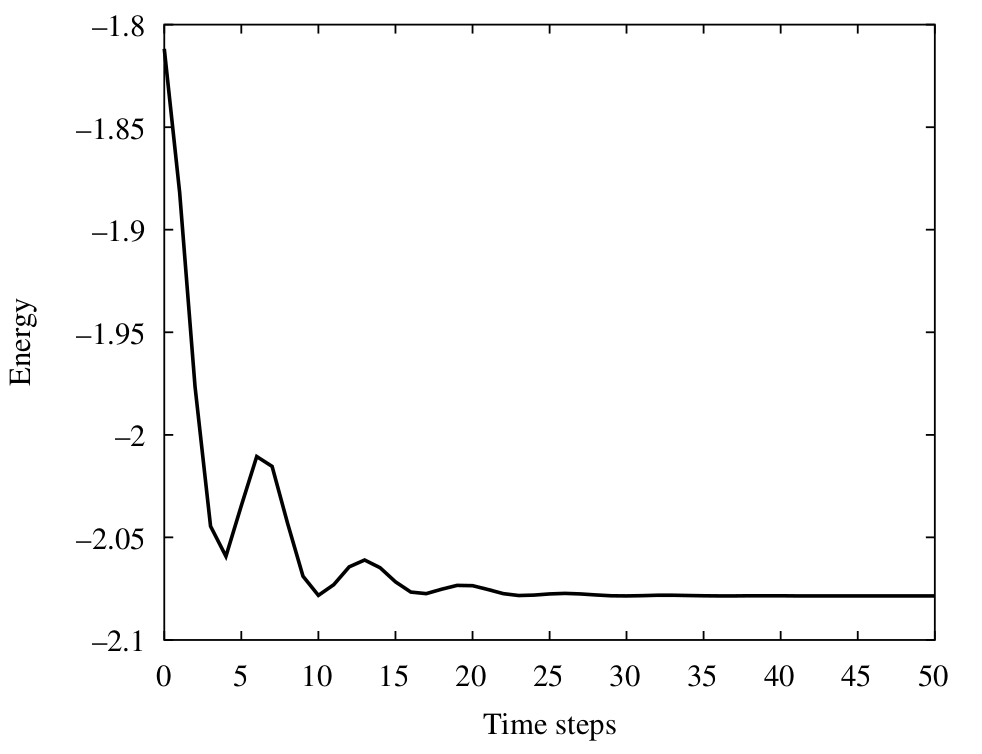
\includegraphics[height=2.1in,width=2.3in,viewport=0 0 740 600,clip]{Figures/Ab-initio-Ene.png}
%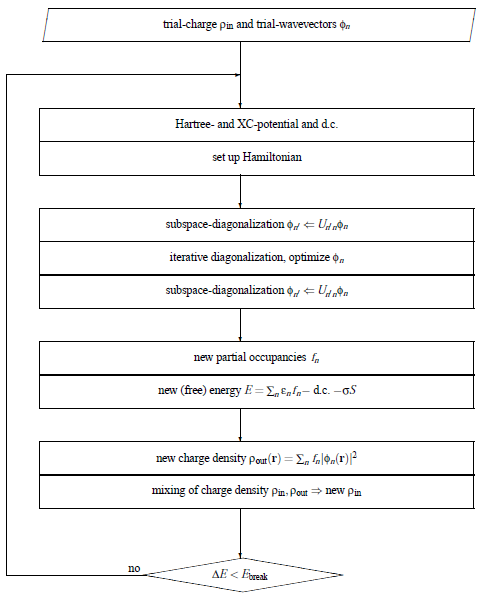
\includegraphics[height=2.75in,width=2.5in,viewport=0 0 480 630,clip]{Figures/VASP_procedure.png}
%\caption{\tiny \textrm{The Flow of calculation for the KS-ground states.}}%(与文献\cite{EPJB33-47_2003}图1对比)
%\label{PAW_baiseset}
%\end{figure} 
%}

\frame
{
	\frametitle{\textrm{VASP}计算的并行效率}
%与同类型软件相比,\textrm{VASP}有着优异的并行能力
	在高性能计算环境下,\textrm{VASP}的并行上限可以突破\textrm{256}核,但当并行核数超过百核数量级,并行效率下降非常明显
\begin{figure}[h!]
	\vspace{-0.10in}
\centering
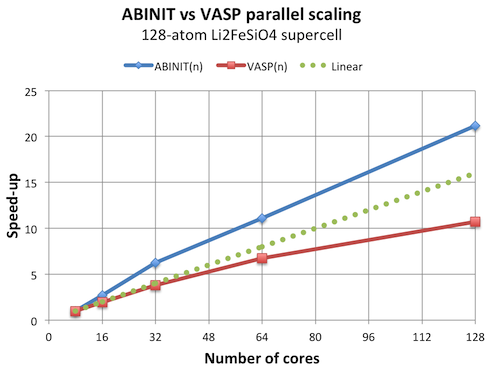
\includegraphics[height=2.35in,width=3.55in,viewport=0 0 240 180,clip]{Figures/VASP-abinit_Li128-1.png}
%\caption{\tiny \textrm{The comparison of parallel scaling for ABINIT vs VASP.}}%(与文献\cite{EPJB33-47_2003}图1对比)
\label{ABINIT_vs_VASP-2}
\end{figure} 
}

\frame
{
	\frametitle{\textrm{VASP}的主要瓶颈:~内存和通信}
\begin{itemize}
	\item 随着计算对象原子数增加,波函数、电子密度和\textrm{Hamiltonian}矩阵等变量存储所需的内存迅速增长
	\item 计算过程中需要完成大量的\textrm{FFT}计算\\
		{\fontsize{7.2pt}{5.2pt}\selectfont{并行核数增加,完成\textrm{FFT}计算的通信量增长更快}}
\end{itemize}
\begin{figure}[h!]
	\vspace{-0.20in}
\centering
%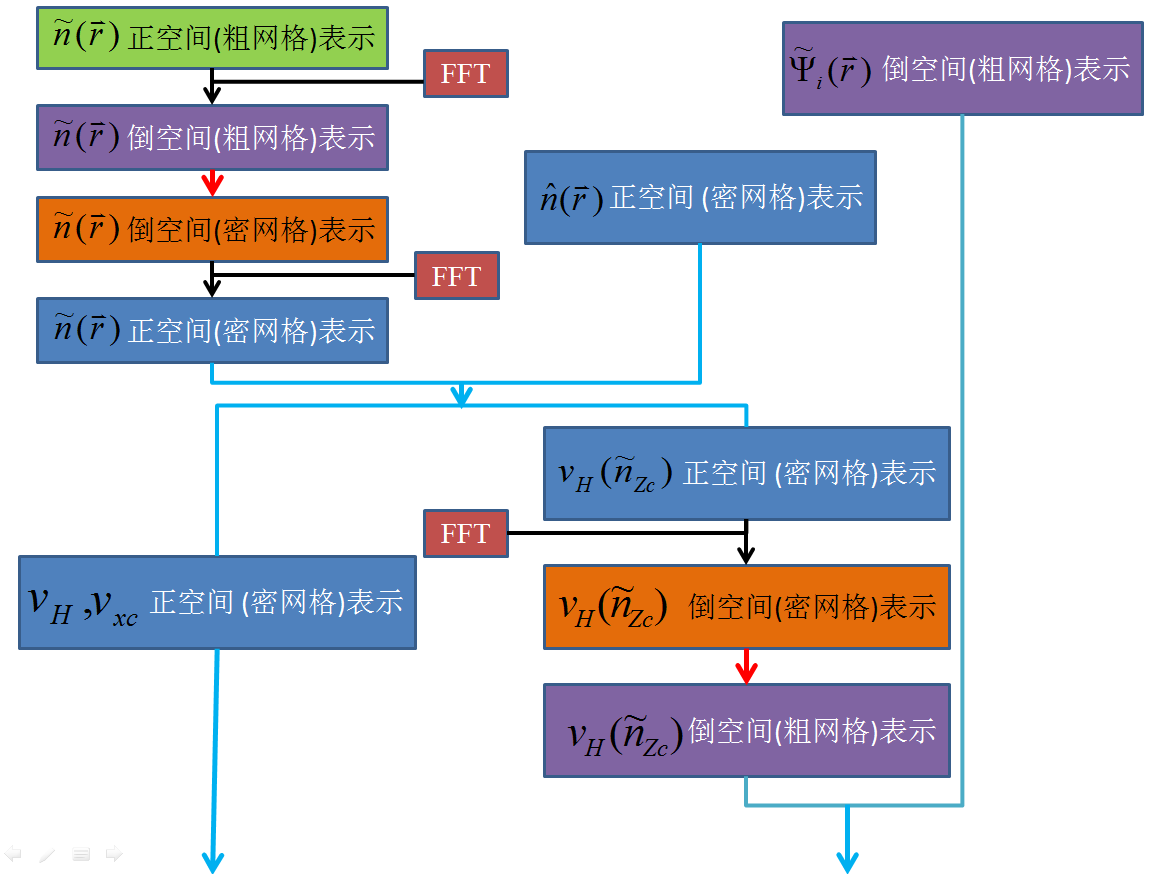
\includegraphics[height=2.7in,width=4.0in,viewport=0 0 1180 875,clip]{Figures/dual_grid.png}
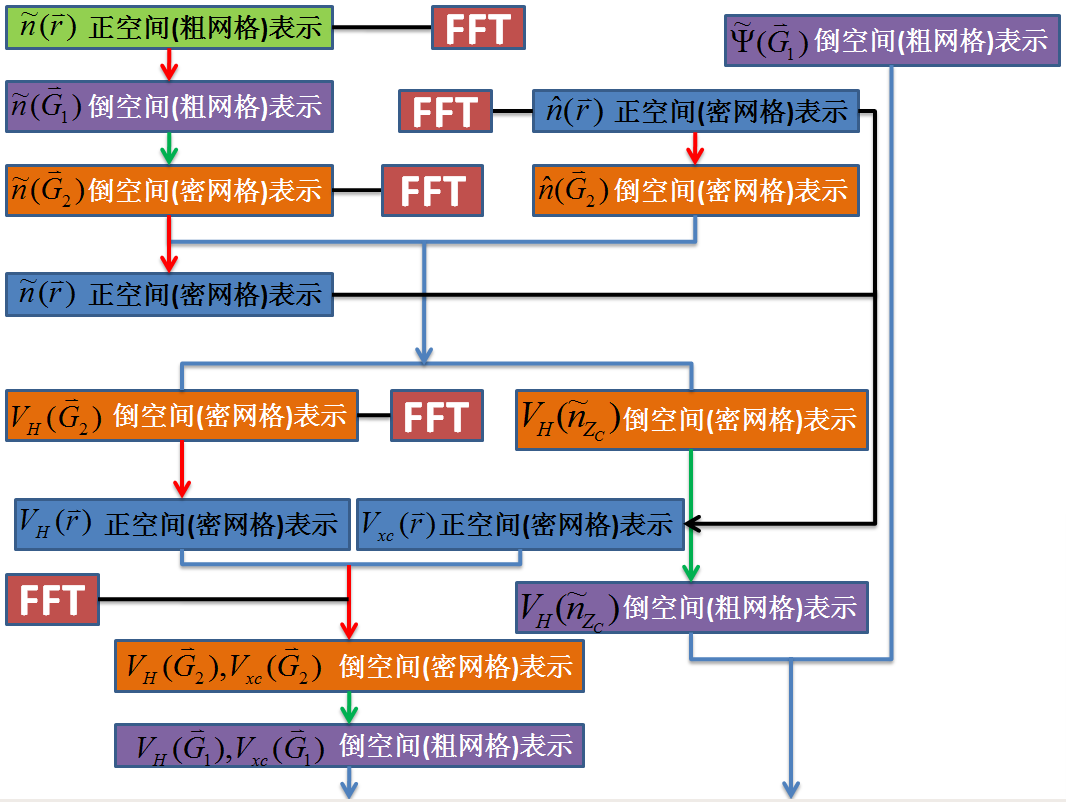
\includegraphics[height=1.39in,width=1.98in,viewport=0 0 800 600,clip]{Figures/dual_grid-2.png}
%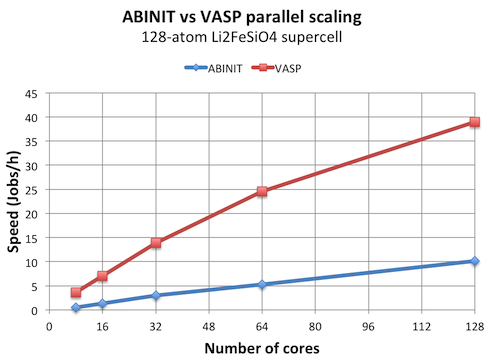
\includegraphics[height=1.55in,width=1.95in,viewport=0 0 240 200,clip]{Figures/VASP-abinit_Li128-2.png}
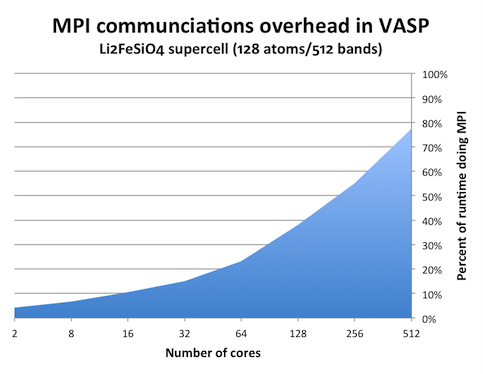
\includegraphics[height=1.55in,width=1.95in,viewport=0 0 240 200,clip]{Figures/VASP-mpi-Li128.png}
%\caption{\tiny \textrm{The comparison of parallel scaling for ABINIT vs VASP.}}%(与文献\cite{EPJB33-47_2003}图1对比)
\label{ABINIT_vs_VASP-3}
\end{figure} 
\textrm{VASP}计算$10^2$原子量级的体系问题不大,\textcolor{red}{但计算$10^3$原子量级规模的体系异常吃力}
%对并行系统与\textrm{VASP}结合作深度改造(如国家超算天津中心方案),\textrm{VASP}的并行扩展可以到$10^4$核级别,这一改造需要对底层代码和计算框架作较大规模改动

}

\frame
{
	\frametitle{\textrm{VASP}的\textrm{GPU}加速}
\textrm{NVIDIA}多年来致力于\textrm{VASP}的\textrm{GPU}加速,取得了一定的效果,但仍比较有限
\begin{itemize}
	\item \textrm{GPU}加速对于分子动力学计算特别有效
	\item 稠密的矩阵-向量乘计算,限制了\textrm{GPU}加速在第一原理计算中应用
	\item 通用配置下,\textrm{GPU}对\textrm{VASP}计算平均加速效果,提升\textrm{4$\sim$6}倍
\end{itemize}
\begin{figure}[h!]
	\vspace{-0.15in}
\centering
%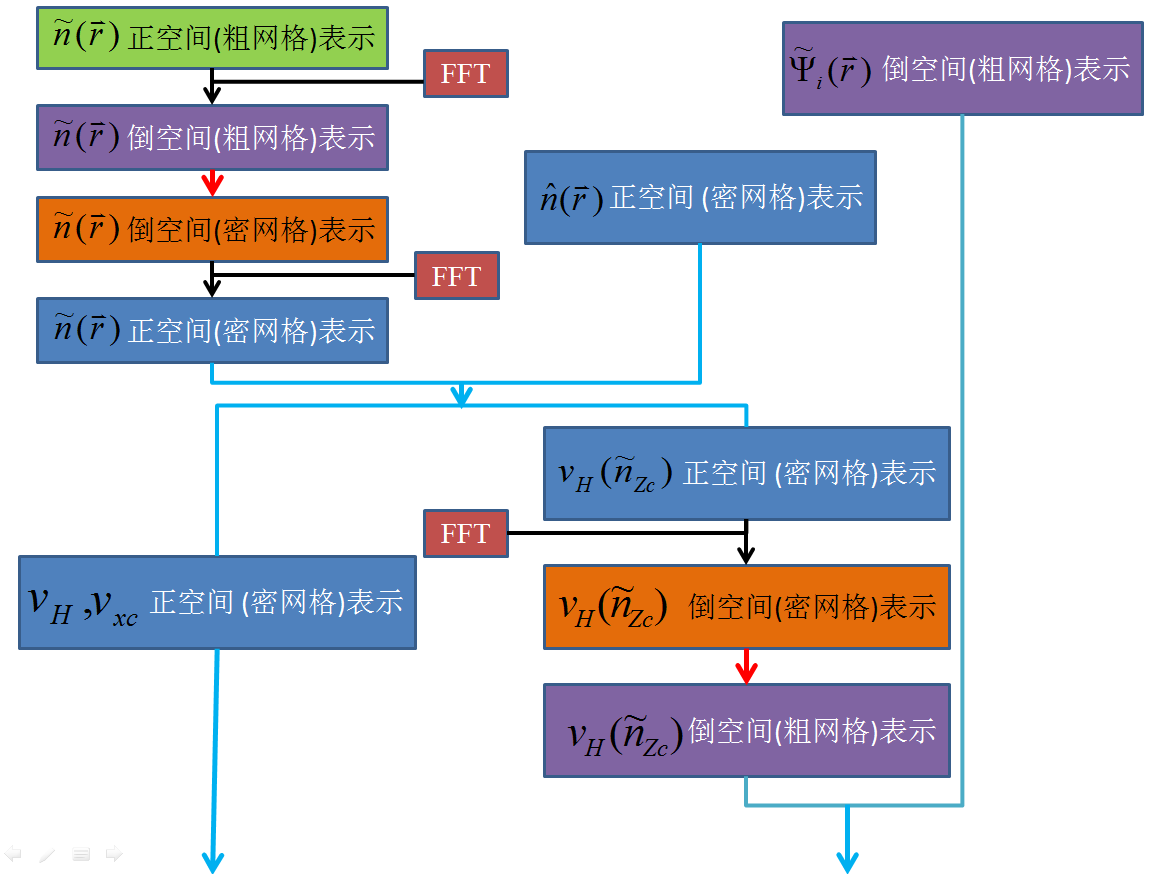
\includegraphics[height=2.7in,width=4.0in,viewport=0 0 1180 875,clip]{Figures/dual_grid.png}
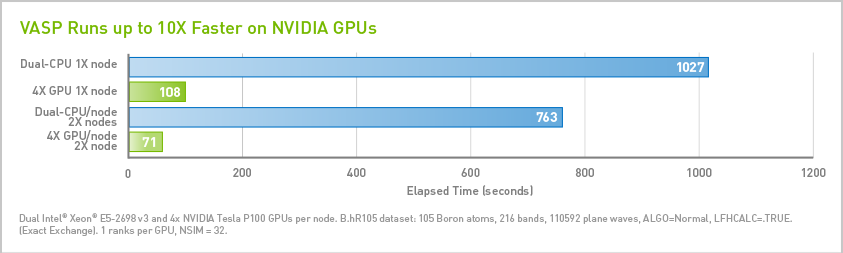
\includegraphics[height=1.2in,width=4.05in,viewport=0 0 850 260,clip]{Figures/VASP-GPU-CPU.png}
%\caption{\tiny \textrm{Compare of VASP calculation with GPU and CPU.}}%(与文献\cite{EPJB33-47_2003}图1对比)
\label{VASP_GPU}
\end{figure} 
	\vspace{-0.15in}
\textcolor{red}{\textrm{GPU}加速不是提升\textrm{VASP}计算规模的最有效方案}
}

\section{针对\rm{VASP}计算能力的提升策略}
\begin{frame}
	\frametitle{\textrm{VASP}中的矩阵-向量乘}
	大规模\textrm{DFT}计算面临的效率问题,根源在于系统软件平台\\
	{\fontsize{7.2pt}{5.2pt}\selectfont{传统系统软件平台难以充分发挥硬件性能,无法为\textrm{DFT}计算软件提供高效适配与支持}}
	\vskip 3pt 
\textrm{VASP}软件将大模型的计算转化成矩阵基础操作\\
{\fontsize{7.2pt}{5.2pt}\selectfont{迭代对角化方案,依次(近似)求解矩阵本征值,因此单个本征值求解过程中,矩阵计算的相关性极高,参与计算的\textrm{CPU}核之间存在非常频繁的通信,产生极大的通信压力}}
	\begin{itemize}
		\item 如果配置较多本征值并行处理,则需要更多的系统资源来对多个本征值计算进行描述,模型越大,冗余开销越大\\
			{\fontsize{7.2pt}{5.2pt}\selectfont{可能影响实用性,甚至超过了现有计算机集群的处理极限}}
		\item 如果把大量系统资源配置到单一本征值,则会因算法失去局部性,各\textrm{CPU}核之间计算任务耦合过重\\
	{\fontsize{7.2pt}{5.2pt}\selectfont{可能造成系统过载}}
	\end{itemize}
	基于通用硬件搭建,通过优化系统软件层面对\textrm{DFT}计算的支持,释放\textrm{VASP}等软件的并行计算潜力,实现更大规模\textrm{DFT}模型的高效支持
\end{frame}

\begin{frame}
	\frametitle{主要技术难点}
	提升单个本征值求解的矩阵-向量乘处理极限,最大程度集成单个本征值计算的资源投入
	\begin{itemize}
		\item 高通量的分布式矩阵运算,会导致频繁的系统通信,在系统软件的临界区会产生严重冲突\\
			{\fontsize{7.2pt}{5.2pt}\selectfont{例如,多个计算节点同时请求访问共享资源、传输关键数据时,频繁的竞争与等待使得数据传输延迟大幅增加}}
%构造一种新型通讯机制,兼容\textrm{DFT}计算的高通量矩阵需求与软件环境特征
		\item \textrm{VASP}软件基于\textrm{Intel}等基础库函数支持的并行计算库,在高并行度条件时,暴露出各种不适应\\
			{\fontsize{7.2pt}{5.2pt}\selectfont{例如,某些矩阵运算算法在多核心并行计算时,数据划分与同步机制不合理,导致核心间负载不均衡,大量核心处于空闲等待状态;部分通信算法在高并发数据传输时,因协议设计缺陷引发数据拥塞}}
%			建立科学的算法评估体系,对这类不适用于高并行度的算法进行精准识别,并结合\textrm{DFT}计算特点,设计出适合高并行度的等效实现方案,从算法层面提升\textrm{VASP}软件在大规模并行计算中的性能表现
		\item \textrm{DFT}计算的核心数据结构的空间复杂度偏高\\
			{\fontsize{7.2pt}{5.2pt}\selectfont{\textrm{VASP}的部分核心数据结构的空间复杂度与$n^2$或$n^3$相关,当模型规模逐步扩大达到一定程度时,对于内存储器的开销过大,即使整个集群的\textrm{CPU}核只用于处理一个本征态所需的矩阵运算,仍会面临所需内存不足的问题}}
	\end{itemize}
\end{frame}

\begin{frame}
	\frametitle{总体技术路线}
	自研的虚拟机技术,将硬件进行重新封装,通过一系列自研数据结构、算法与特定编程方法,改变硬件呈现的特性,面向高通量数据处理软件提供更高效的运行环境
	\begin{itemize}
		\item 高通量并发计算系统:~解决单一本征值计算过程矩阵运算的\textrm{CPU}核之间高效配合的问题
			\begin{enumerate}
\fontsize{7.2pt}{5.2pt}\selectfont
				\item 重新划分软件分层
				\item 严格控制临界区范围
				\item 与高通量通信硬件的深度适配
			\end{enumerate}
		\item 并行计算库:~与高通量通信硬件的深度适配
			\begin{itemize}
\fontsize{7.2pt}{5.2pt}\selectfont
				\item 数据处理分层化:~将部分计算任务的处理过程进行分层,在负载均担与实时性需求之间进行再平衡
				\item 计算去中心化:~去掉各种形式的``主结点'',部分算法进行``去中心化''重写
			\end{itemize}
		\item 内存溢出子系统:~%在计算机集群系统中,
			集成内存储器的规模超过一定范围后,成本会明显增加\\
			{\fontsize{7.2pt}{5.2pt}\selectfont{
				针对\textrm{DFT}运算的核心数据结构访问局部性与连续性,设计了内外存储器联动的算法:~%该算法
		\\精准捕捉数据访问的规律,保证算法执行效率下降不超过\textrm{20\%}的前提下,可处理规模为内存储器\textrm{200\%$\sim$1000\%}以上的数据结构,有效突破内存容量对大规模计算的制约}}
	\end{itemize}
\end{frame}

\section{计算结果}
%\frame
%{
%	\frametitle{对\textrm{VASP}并行优化及计算规模扩容}
%	与其余第一原理计算软件相比,\textrm{VASP}的最大优势
%	\begin{itemize}
%		\item 应用\textrm{PAW}方法,有效处理含有\textit{d}、\textit{f}电子的过渡金属体系
%		\item 提供了多种电子结构和原子受力的优化算法(\textrm{SD}、\textrm{CG}、\textrm{RMM-DIIS}等)
%		\item 用户可通过控制文件\textcolor{blue}{\textrm{INCAR}}的参数调控来选择
%	\end{itemize}
%	由于\textrm{VASP}的计算特点,可以处理的模型原子数目的上限一般是百量级($10^2$),对于复杂体系如合金、化合物和电池材料等,现有的模拟规模是制约\textrm{VASP}软件的重要因素
%	\vskip 1.5pt
%	我们变革了\textrm{VASP}并行方式,%在不改变\textrm{VASP}运行策略基础上
%	实现了计算规模的数量级的扩展
%\begin{figure}[h!]
%\centering
%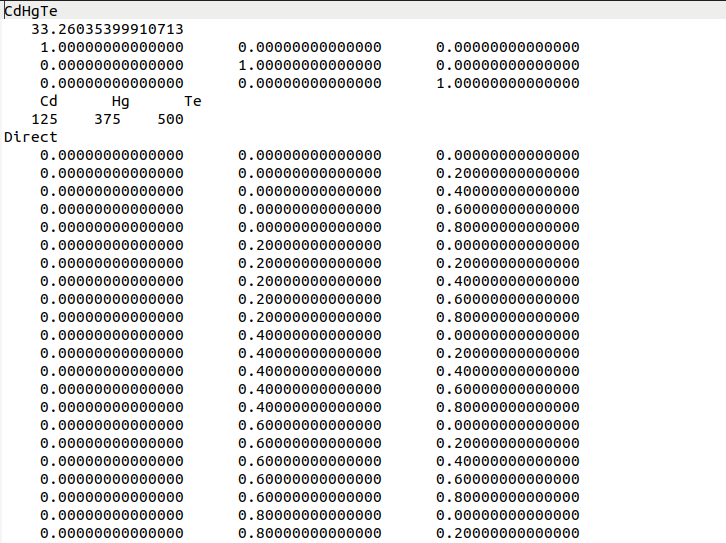
\includegraphics[height=0.85in,width=3.05in,viewport=0 350 726 543,clip]{Figures/VASP_huge_POSCAR.png}
%\caption{\tiny \textrm{千原子合金模型.}}%(与文献\cite{EPJB33-47_2003}图1对比)
%\label{VASP_Model}
%\end{figure} 
%}

\frame
{
	\frametitle{\textrm{VASP}计算规模的扩容:~三类模型}
\begin{figure}[h!]
\centering
\vskip -0.6in
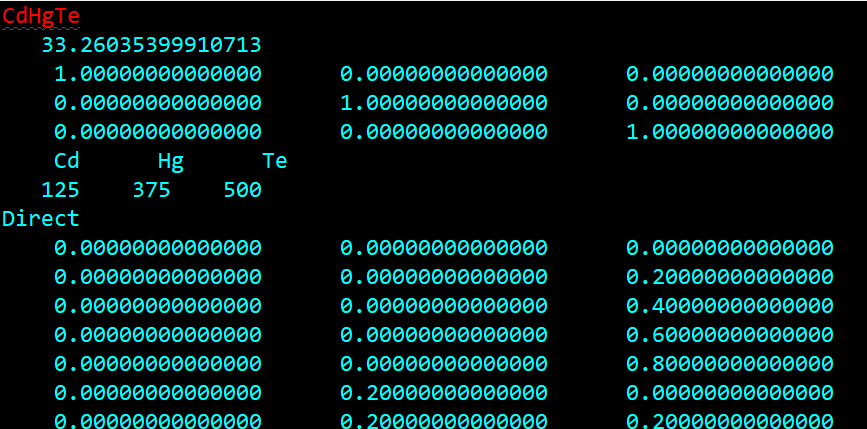
\includegraphics[height=1.45in,width=3.05in,viewport=0 100 656 429,clip]{Figures/VASP_huge_SJTU-CdHgTe_POSCAR.png}
\vskip -0.6in
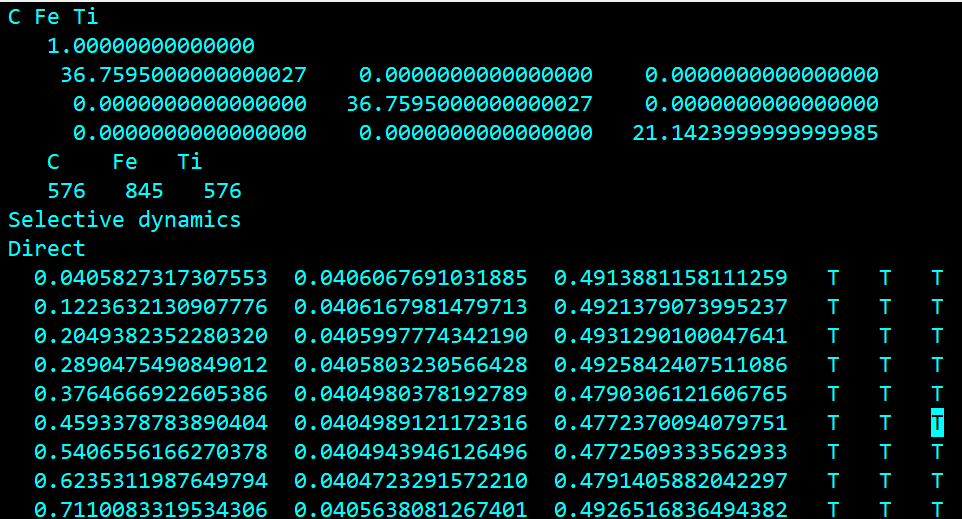
\includegraphics[height=1.65in,width=3.05in,viewport=0 150 726 519,clip]{Figures/VASP_huge_USTB-CFeTi_POSCAR.png}
\vskip -0.05in
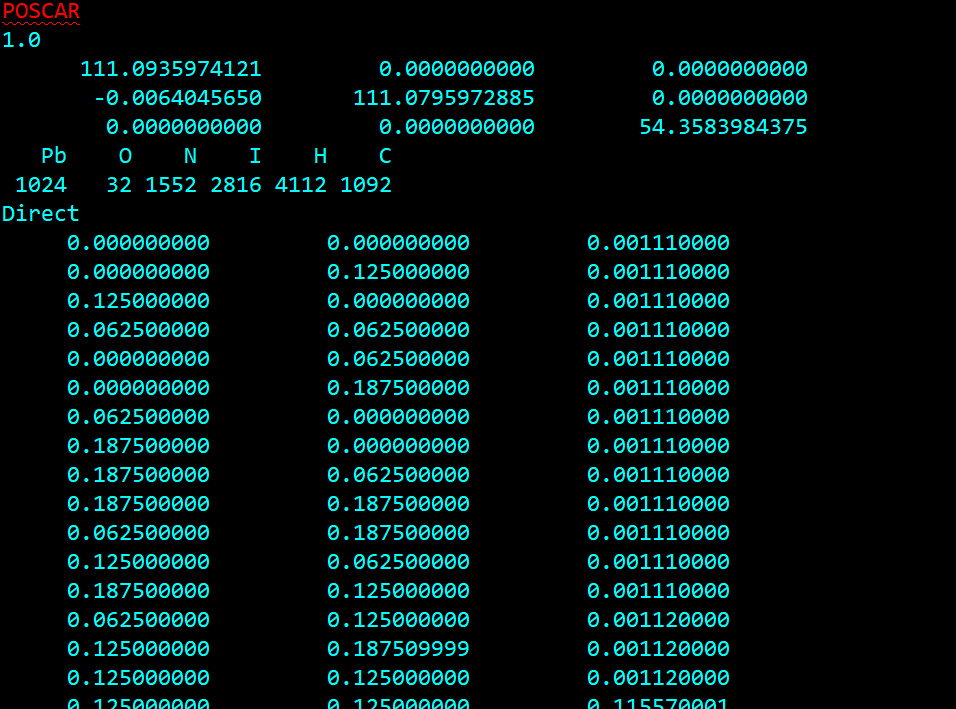
\includegraphics[height=0.95in,width=3.05in,viewport=0 320 680 543,clip]{Figures/VASP_huge_Ningde-PbONICH_POSCAR.png}
\caption{\tiny \textrm{千原子合金模型.}}%(与文献\cite{EPJB33-47_2003}图1对比)
\label{VASP-huge_Model}
\end{figure} 
}

\frame
{
	\frametitle{计算算例:~控制参数}
\begin{figure}[h!]
\centering
\vskip -0.15in
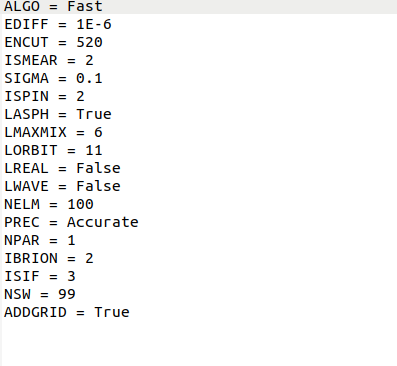
\includegraphics[height=2.75in,width=3.55in,viewport=0 40 397 366,clip]{Figures/VASP_huge_INCAR.png}
%\caption{\tiny \textrm{千原子合金模型:~控制参数\textrm{INCAR}.}}%(与文献\cite{EPJB33-47_2003}图1对比)
\label{VASP_Contral}
\end{figure} 
}

\frame
{
	\frametitle{计算算例:~并行规模}
\begin{figure}[h!]
\centering
\vskip -0.15in
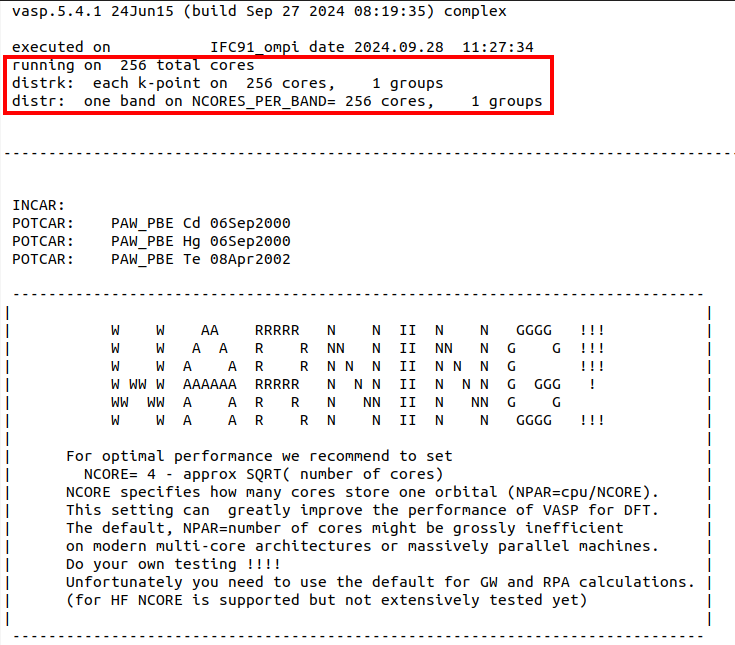
\includegraphics[height=2.75in,width=3.55in,viewport=0 150 735 645,clip]{Figures/VASP_huge_OUTCAR.png}
%\caption{\tiny \textrm{千原子合金模型:~并行规模($\vec k$点:~\textcolor{red}{$2\times2\times2$}).}}%(与文献\cite{EPJB33-47_2003}图1对比)
\label{VASP_Parallel}
\end{figure} 
}

%\frame
%{
%	\frametitle{计算算例:~初始计算效率}
%\begin{figure}[h!]
%\centering
%\vskip -0.15in
%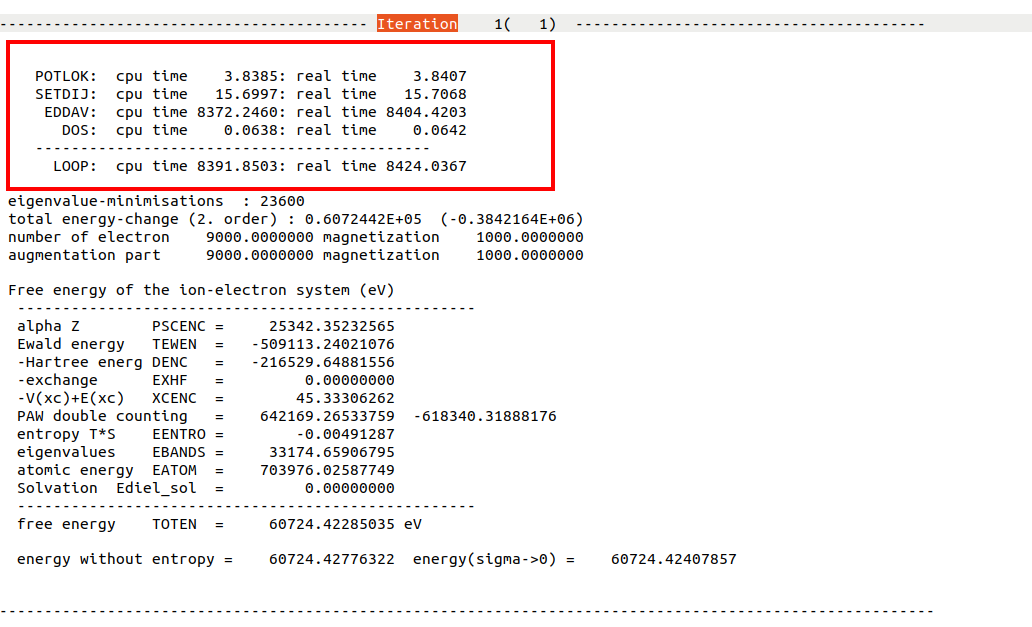
\includegraphics[height=2.75in,width=4.05in,viewport=0 0 1032 627,clip]{Figures/VASP_huge_Iteration-1_1.png}
%\caption{\tiny \textrm{千原子合金模型:~计算效率(初始).}}%(与文献\cite{EPJB33-47_2003}图1对比)
%\label{VASP_Effectivity}
%\end{figure} 
%}
%
%\frame
%{
%	\frametitle{计算算例:~计算效率}
%\begin{figure}[h!]
%\centering
%\vskip -0.15in
%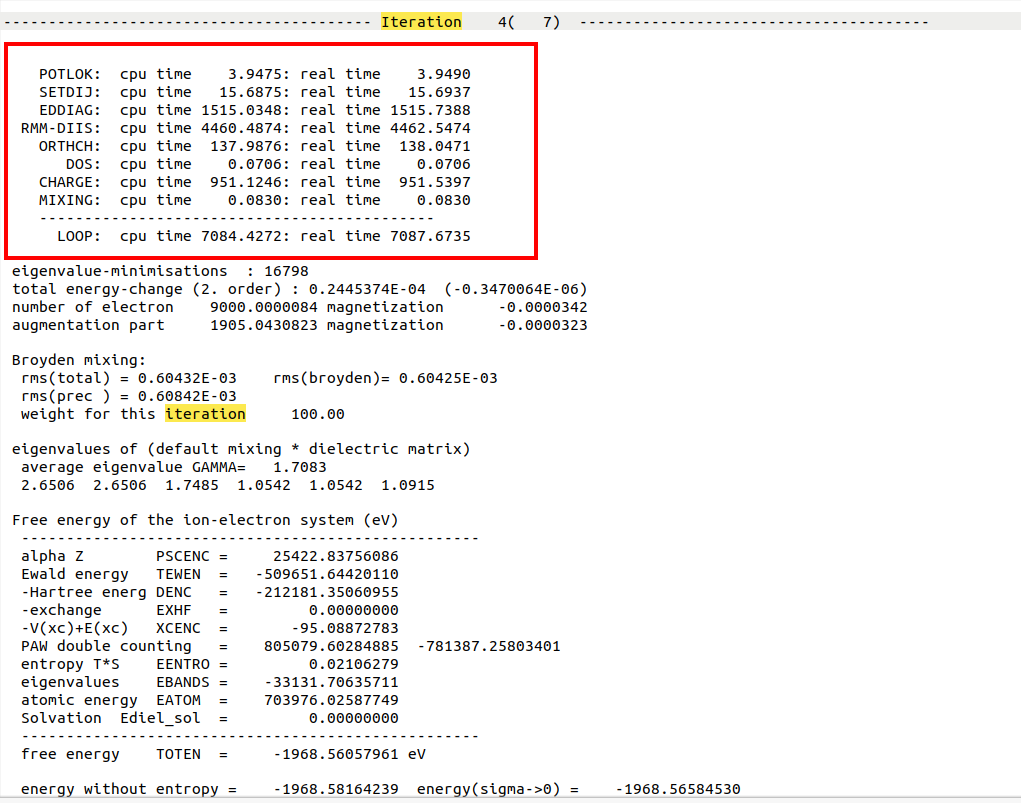
\includegraphics[height=2.75in,width=3.55in,viewport=0 0 1021 803,clip]{Figures/VASP_huge_Iteration-4_7.png}
%\caption{\tiny \textrm{千原子合金模型:~计算效率(稳定).}}%(与文献\cite{EPJB33-47_2003}图1对比)
%\label{VASP_Effectivity-2}
%\end{figure} 
%}
%
%\frame
%{
%	\frametitle{计算算例:~迭代收敛}
%\begin{figure}[h!]
%\centering
%\vskip -0.15in
%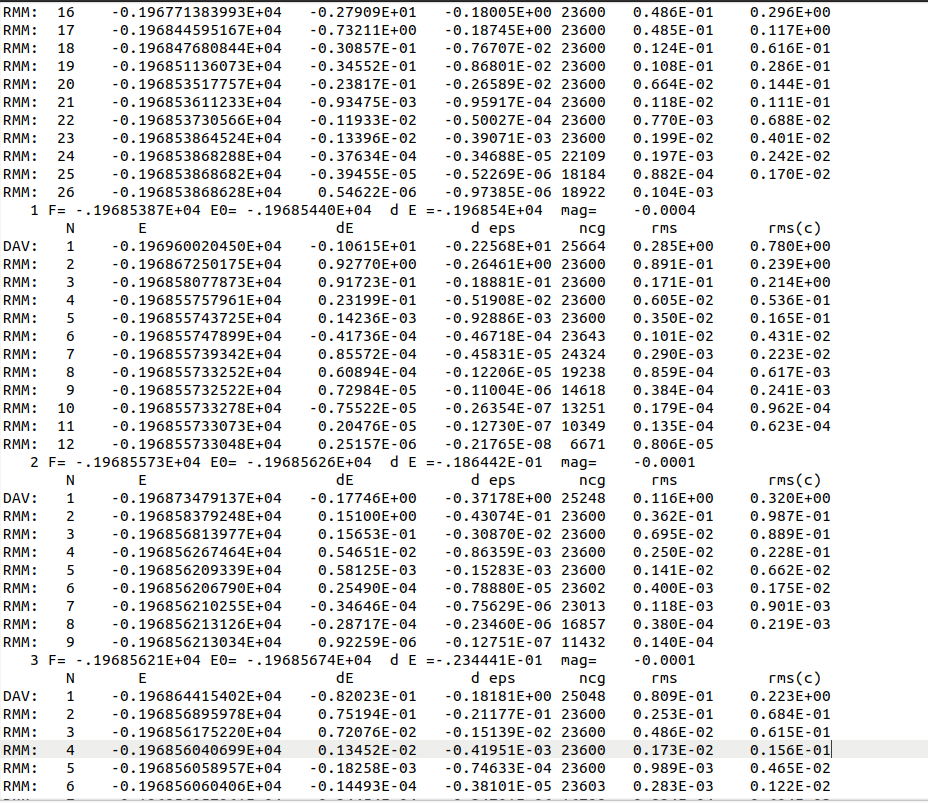
\includegraphics[height=2.75in,width=3.55in,viewport=0 0 928 803,clip]{Figures/VASP_huge_OSZICAR.png}
%\caption{\tiny \textrm{千原子合金模型:~迭代收敛.}}%(与文献\cite{EPJB33-47_2003}图1对比)
%\label{VASP_Convergence}
%\end{figure} 
%}
%
%\frame
%{
%	\frametitle{计算算例}
%\begin{figure}[h!]
%\centering
%\vskip -0.18in
%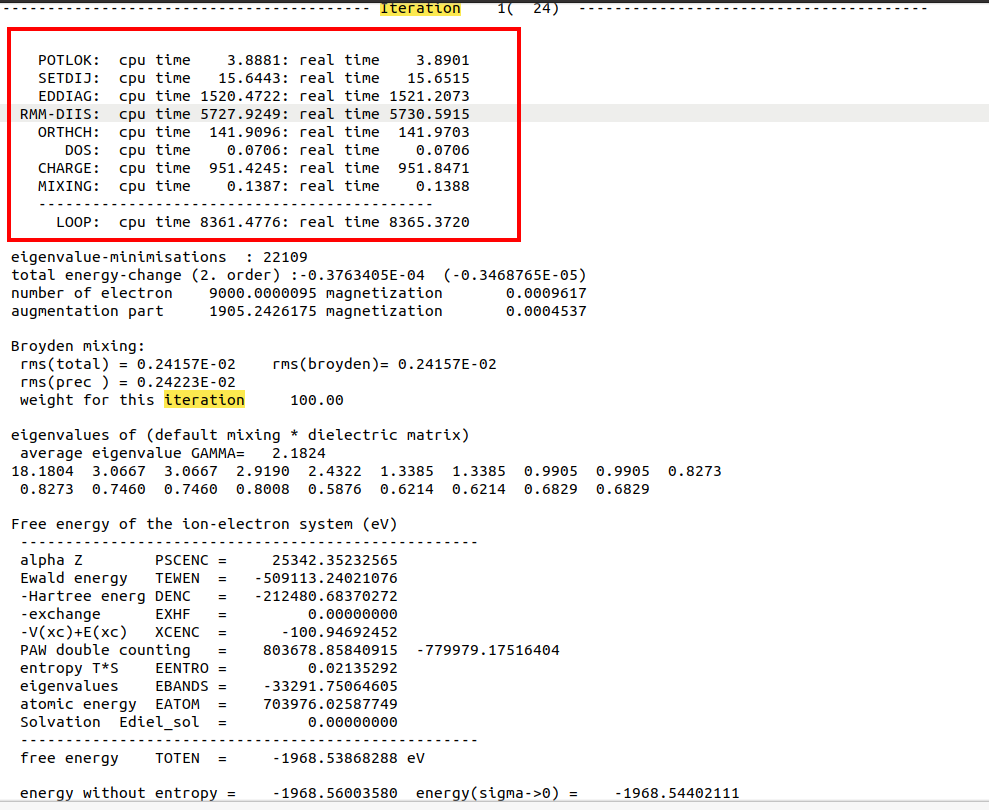
\includegraphics[height=1.35in,width=2.90in,viewport=0 570 589 806,clip]{Figures/VASP_huge_Iteration-1_24.png}
%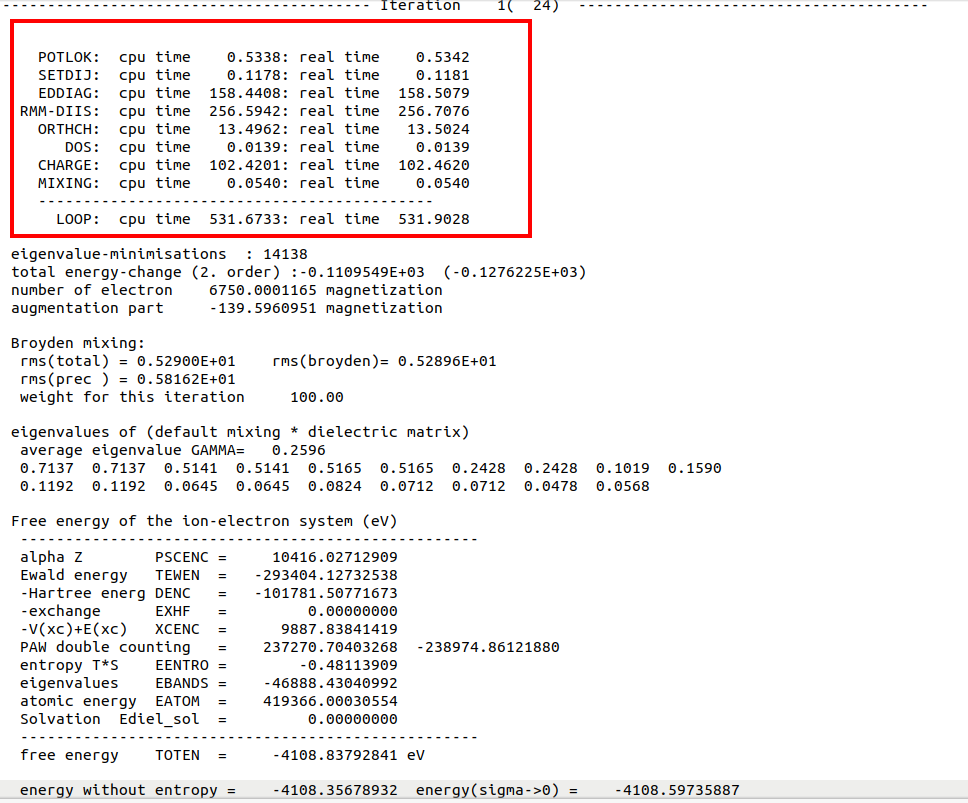
\includegraphics[height=1.35in,width=2.90in,viewport=0 560 568 803,clip]{Figures/VASP_huge_Iteration-1_24-2.png}
%\caption{\tiny \textrm{千原子合金模型($\vec k$点:~\textcolor{red}{$2\times2\times2$} vs~\textcolor{red}{$1\times1\times1$}).}}%(与文献\cite{EPJB33-47_2003}图1对比)
%\label{VASP_Model-2}
%\end{figure} 
%}

\begin{frame}
	\frametitle{计算算例:~\textrm{CFeTi}}
\begin{figure}[h!]
\centering
\vskip -0.41in
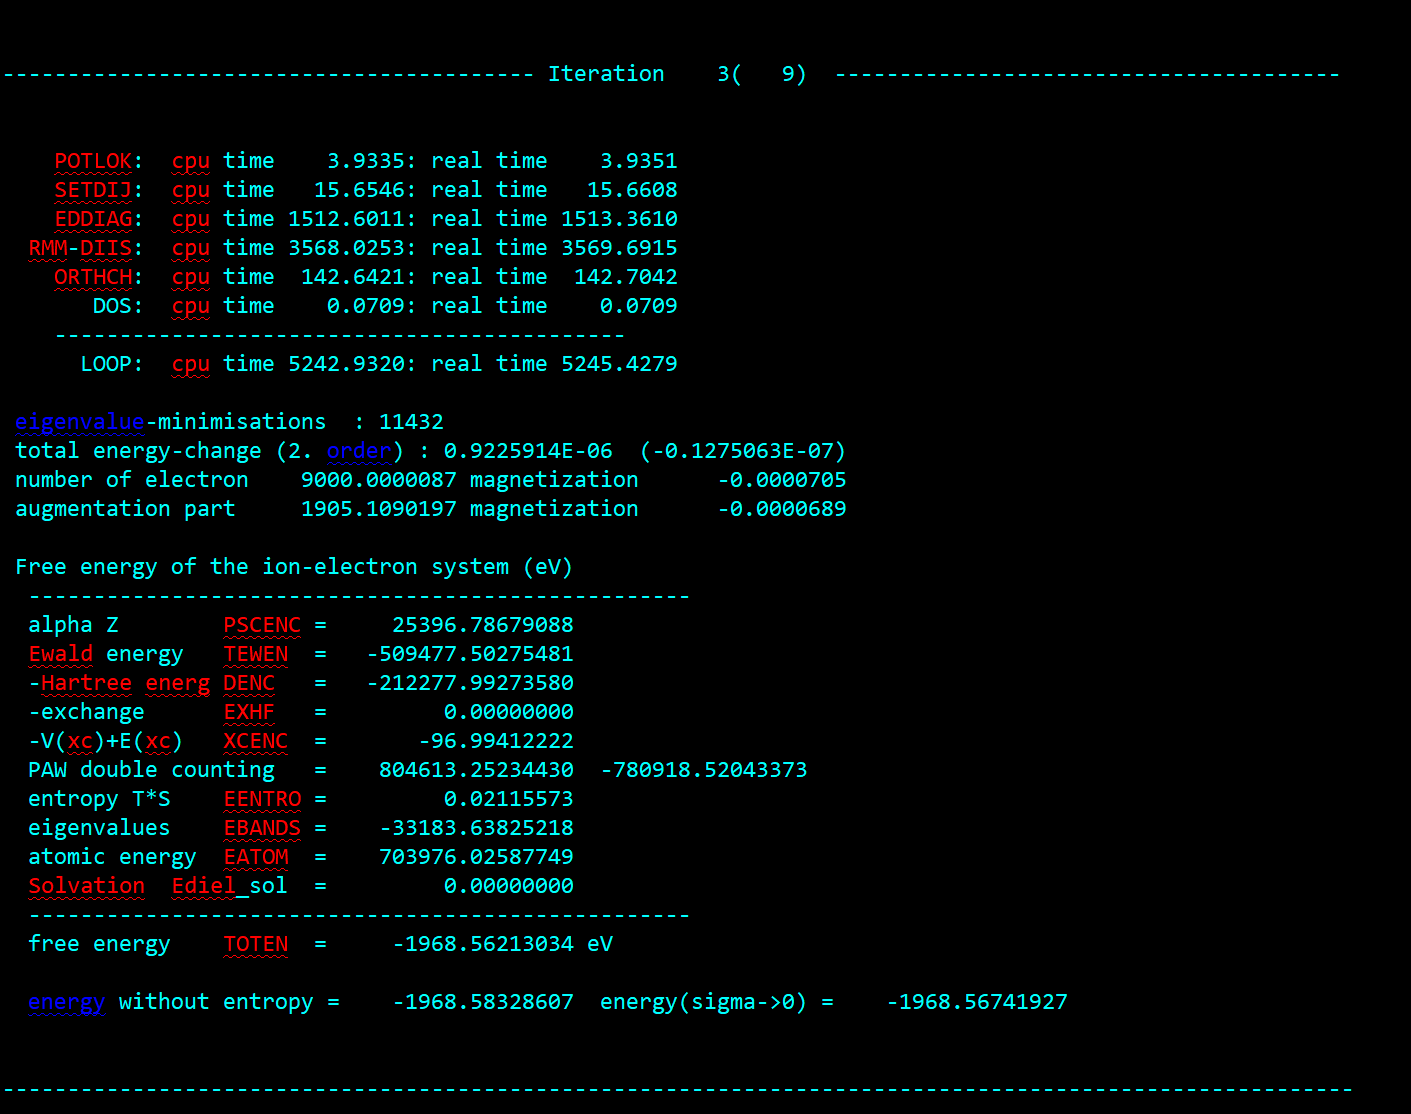
\includegraphics[height=1.05in,width=1.30in,viewport=0 0 1268 805,clip]{Figures/VASP_huge_SJTU-CdHgTe_OUTCAR-1.png}
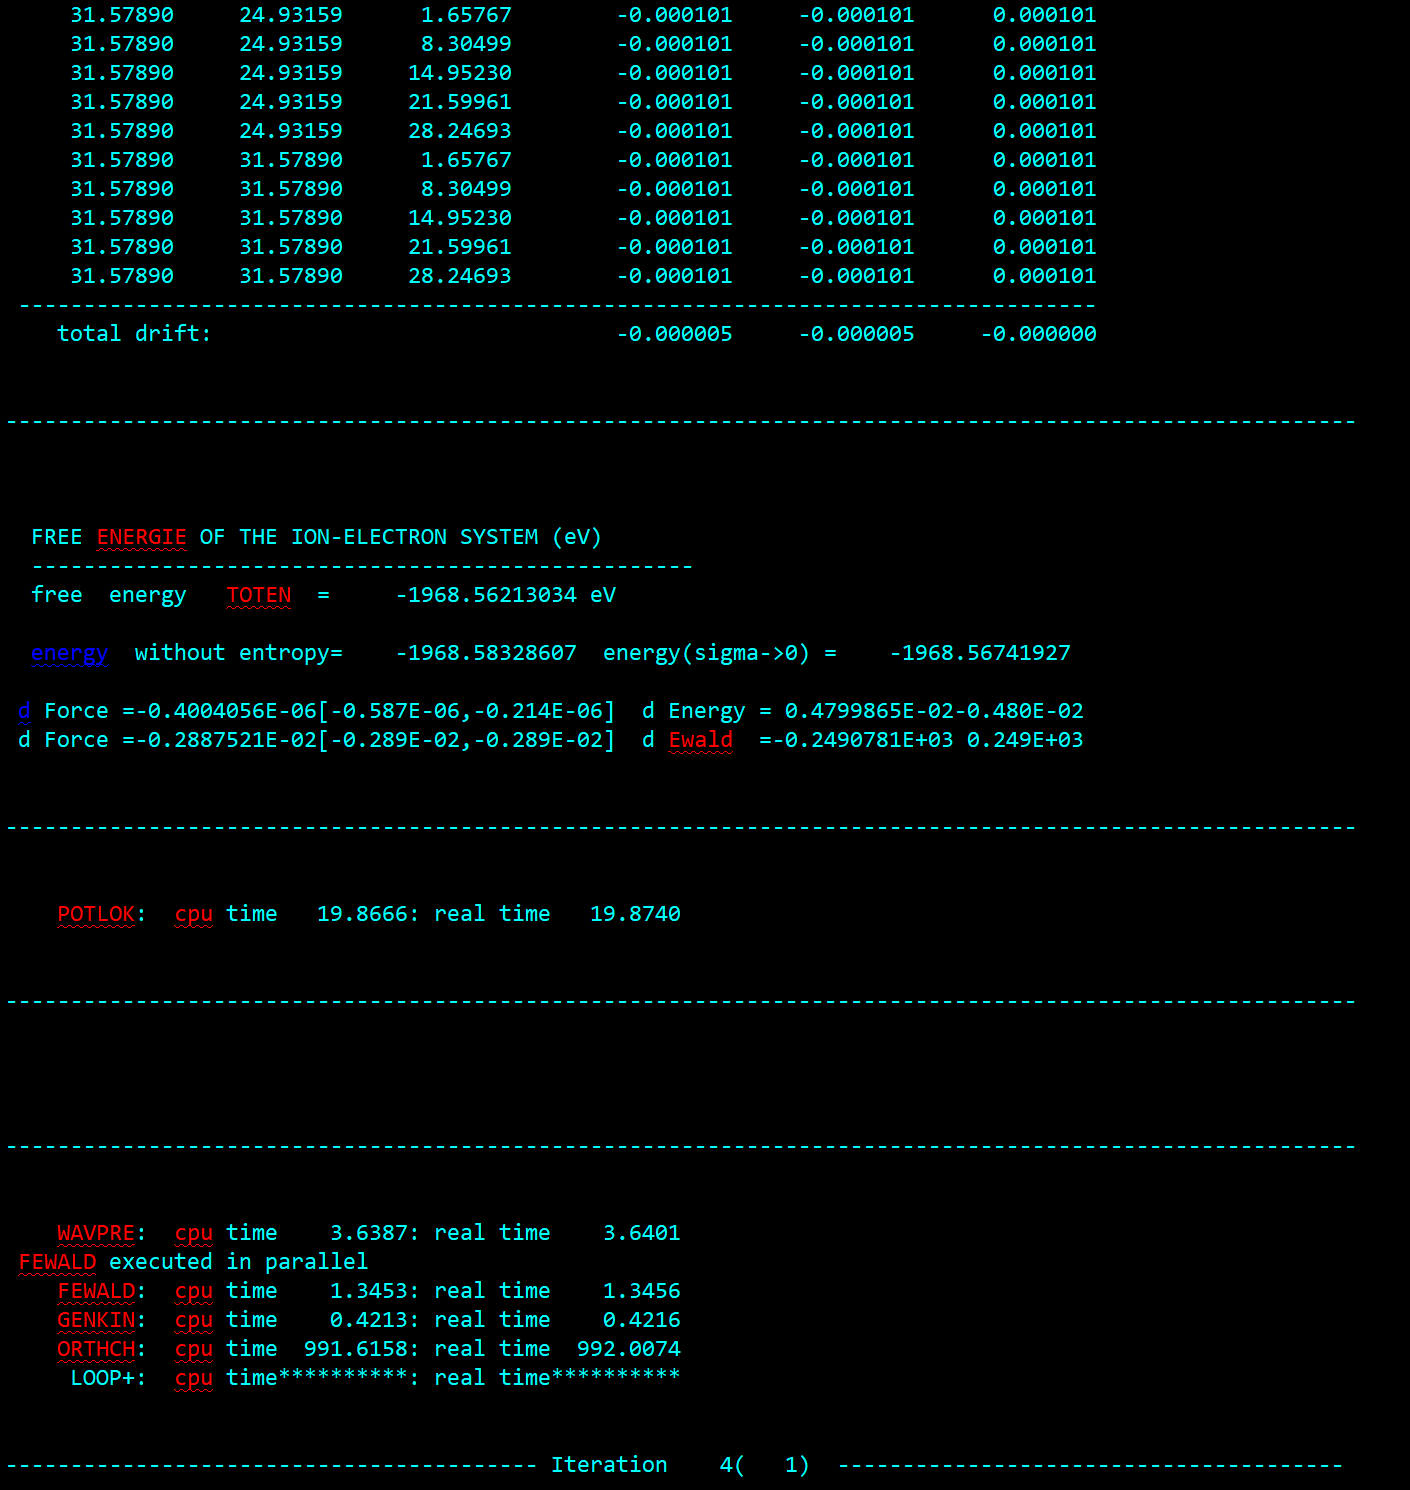
\includegraphics[height=1.55in,width=1.30in,viewport=0 0 1268 1490,clip]{Figures/VASP_huge_SJTU-CdHgTe_OUTCAR-2.png}
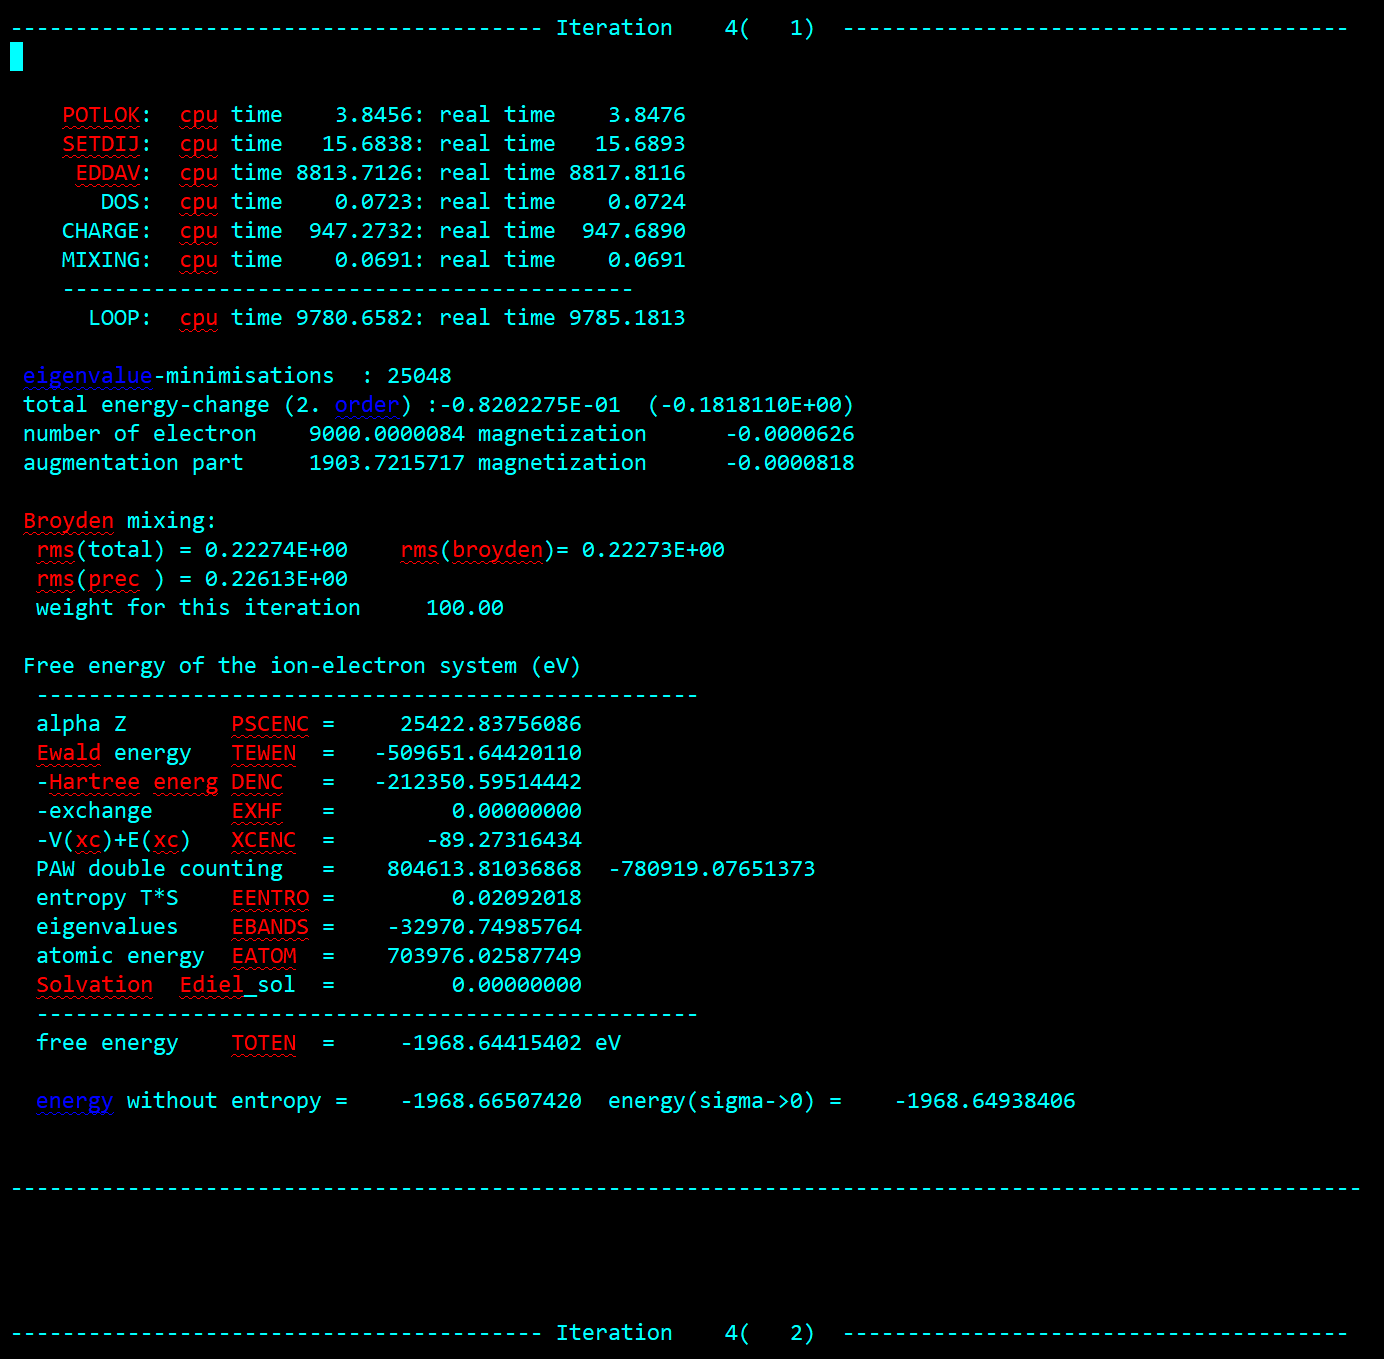
\includegraphics[height=1.55in,width=1.30in,viewport=0 0 1268 1359,clip]{Figures/VASP_huge_SJTU-CdHgTe_OUTCAR-3.png}
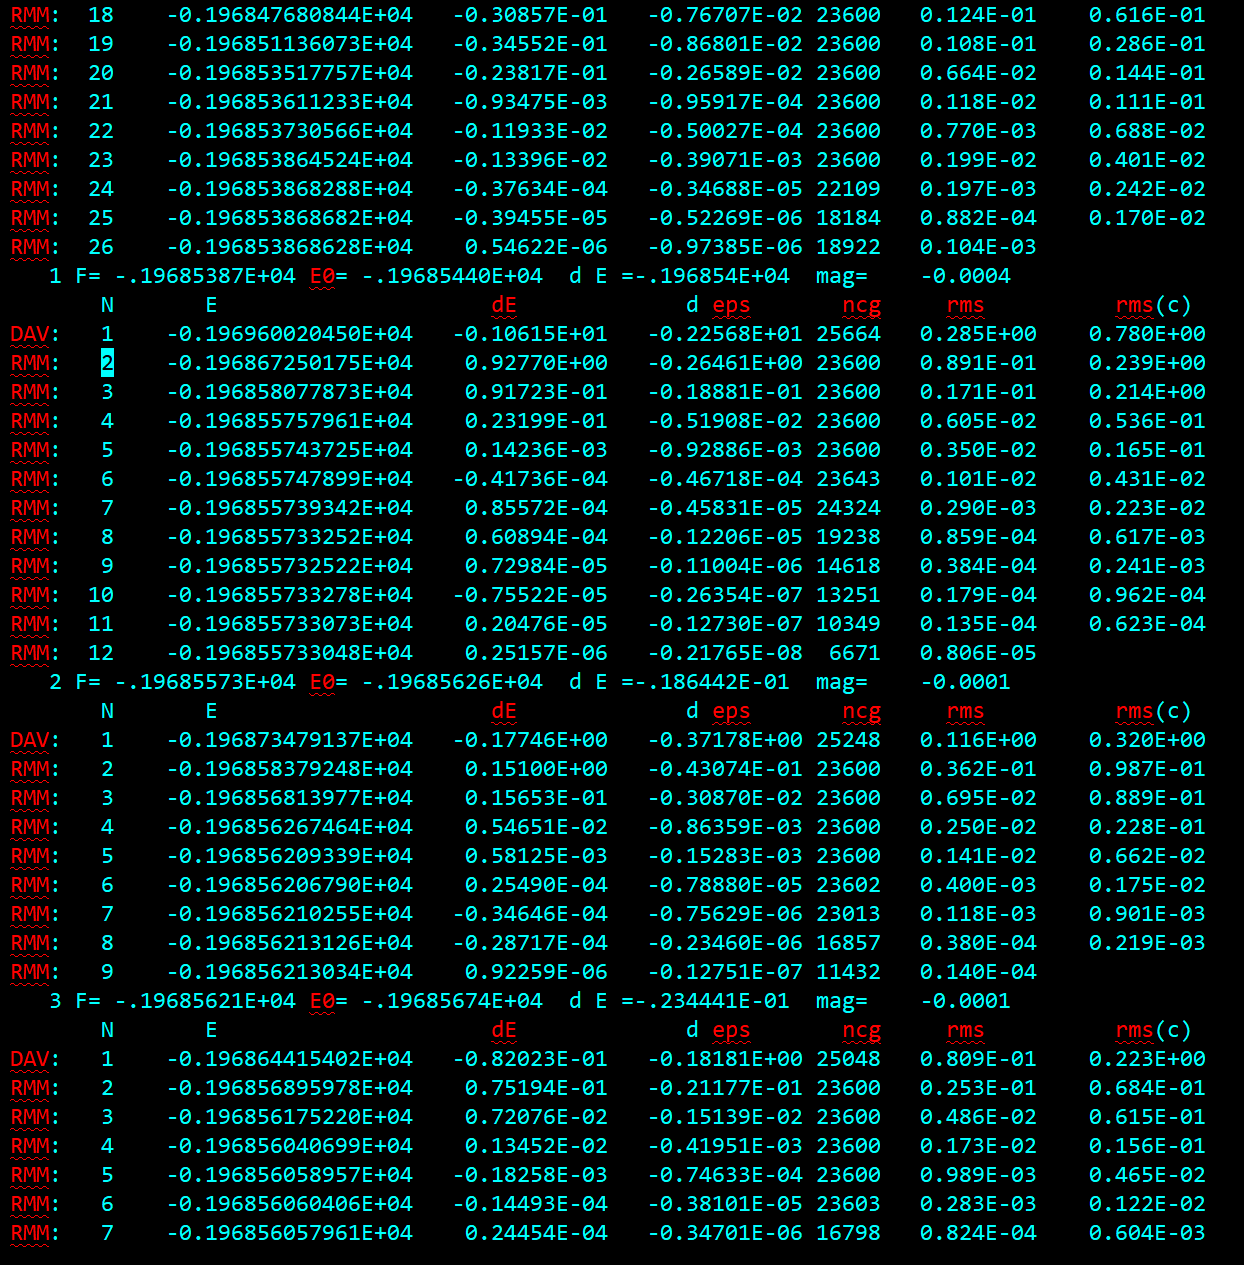
\includegraphics[height=1.55in,width=3.90in,viewport=0 50 1200 650,clip]{Figures/VASP_huge_SJTU-CdHgTe_OSZICAR.png}
%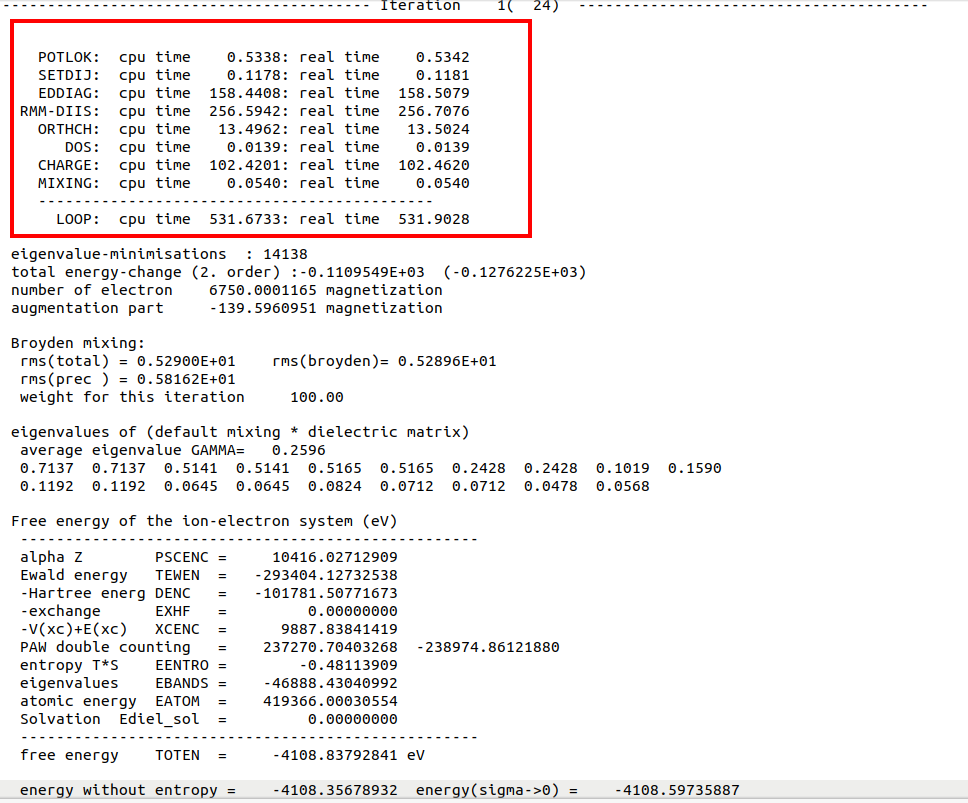
\includegraphics[height=1.35in,width=2.90in,viewport=0 560 568 803,clip]{Figures/VASP_huge_Iteration-1_24-2.png}
%\caption{\tiny \textrm{千原子合金模型($\vec k$点:~\textcolor{red}{$2\times2\times2$} vs~\textcolor{red}{$1\times1\times1$}).}}%(与文献\cite{EPJB33-47_2003}图1对比)
\label{VASP_Model-1}
\end{figure} 
\end{frame}

\begin{frame}
	\frametitle{计算算例:~\textrm{CFeTi}}
\begin{figure}[h!]
\centering
\vskip -0.41in
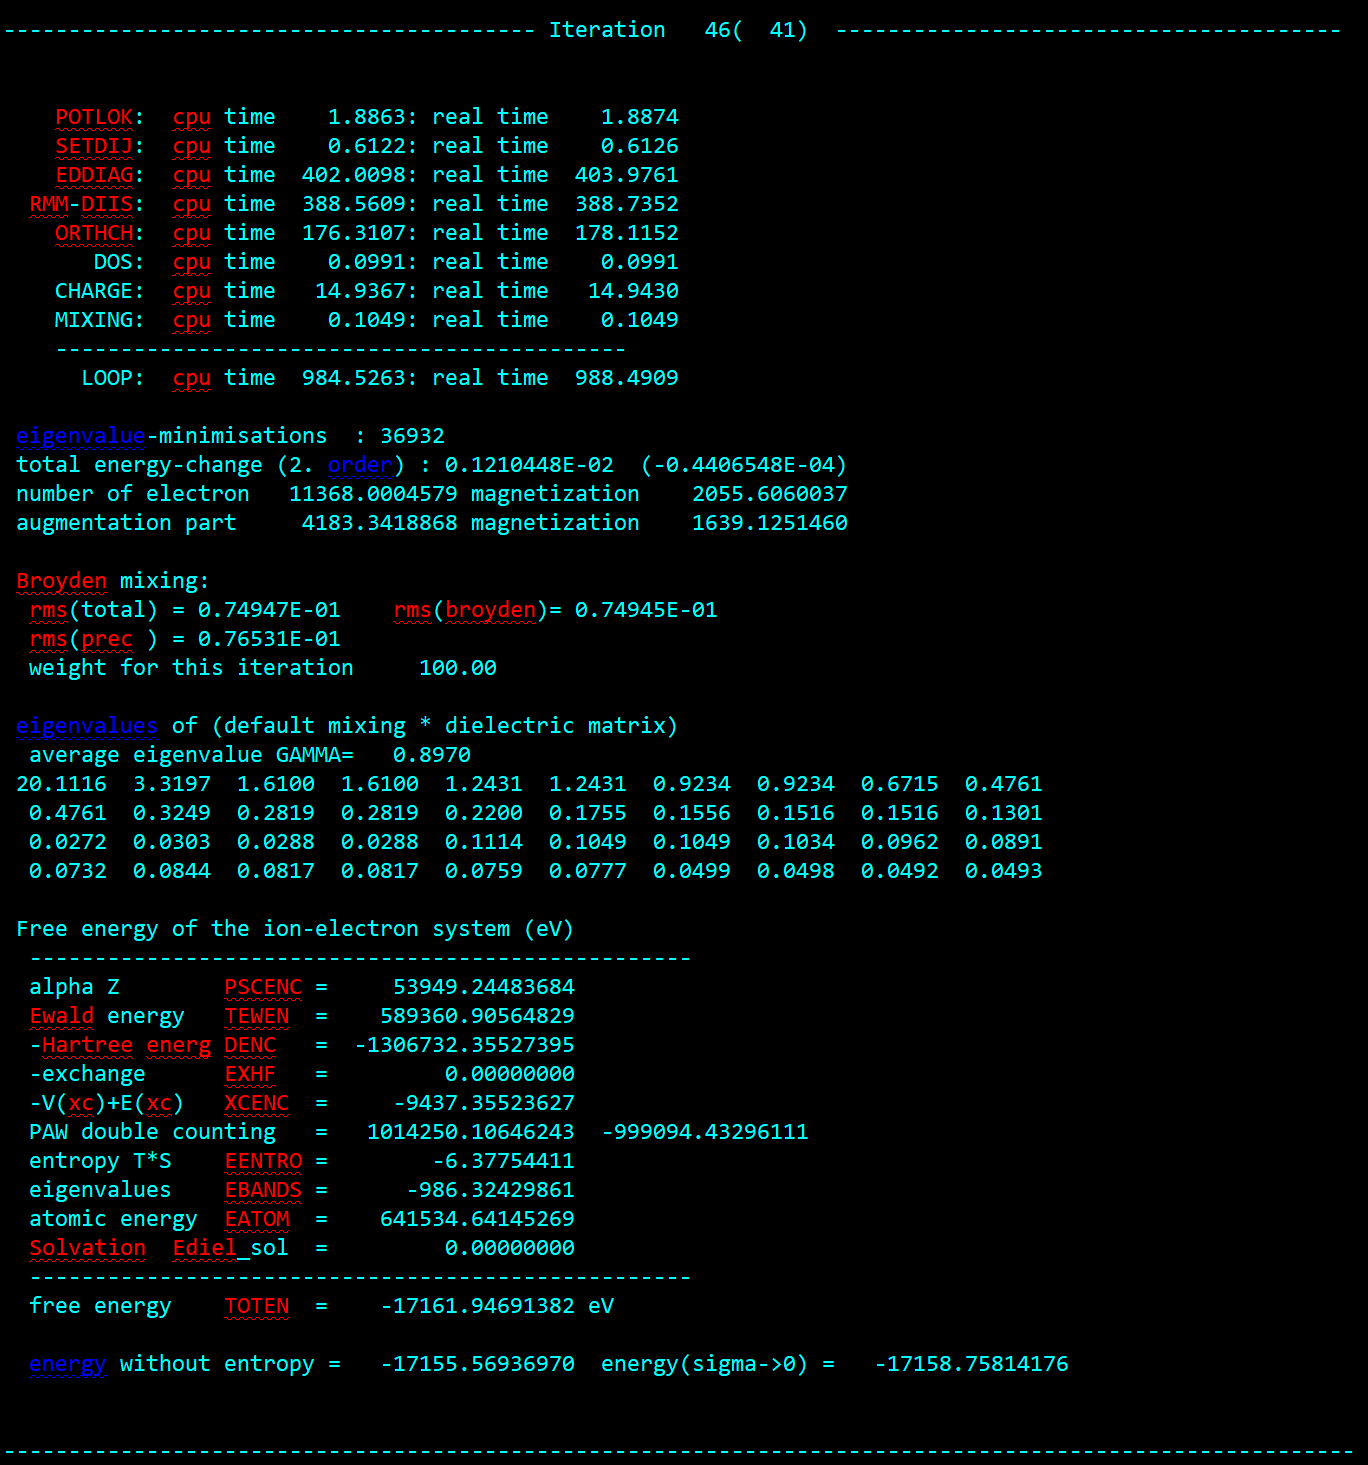
\includegraphics[height=2.15in,width=1.90in,viewport=0 0 1268 1465,clip]{Figures/VASP_huge_USTB-CFeTi_OUTCAR-2.png}
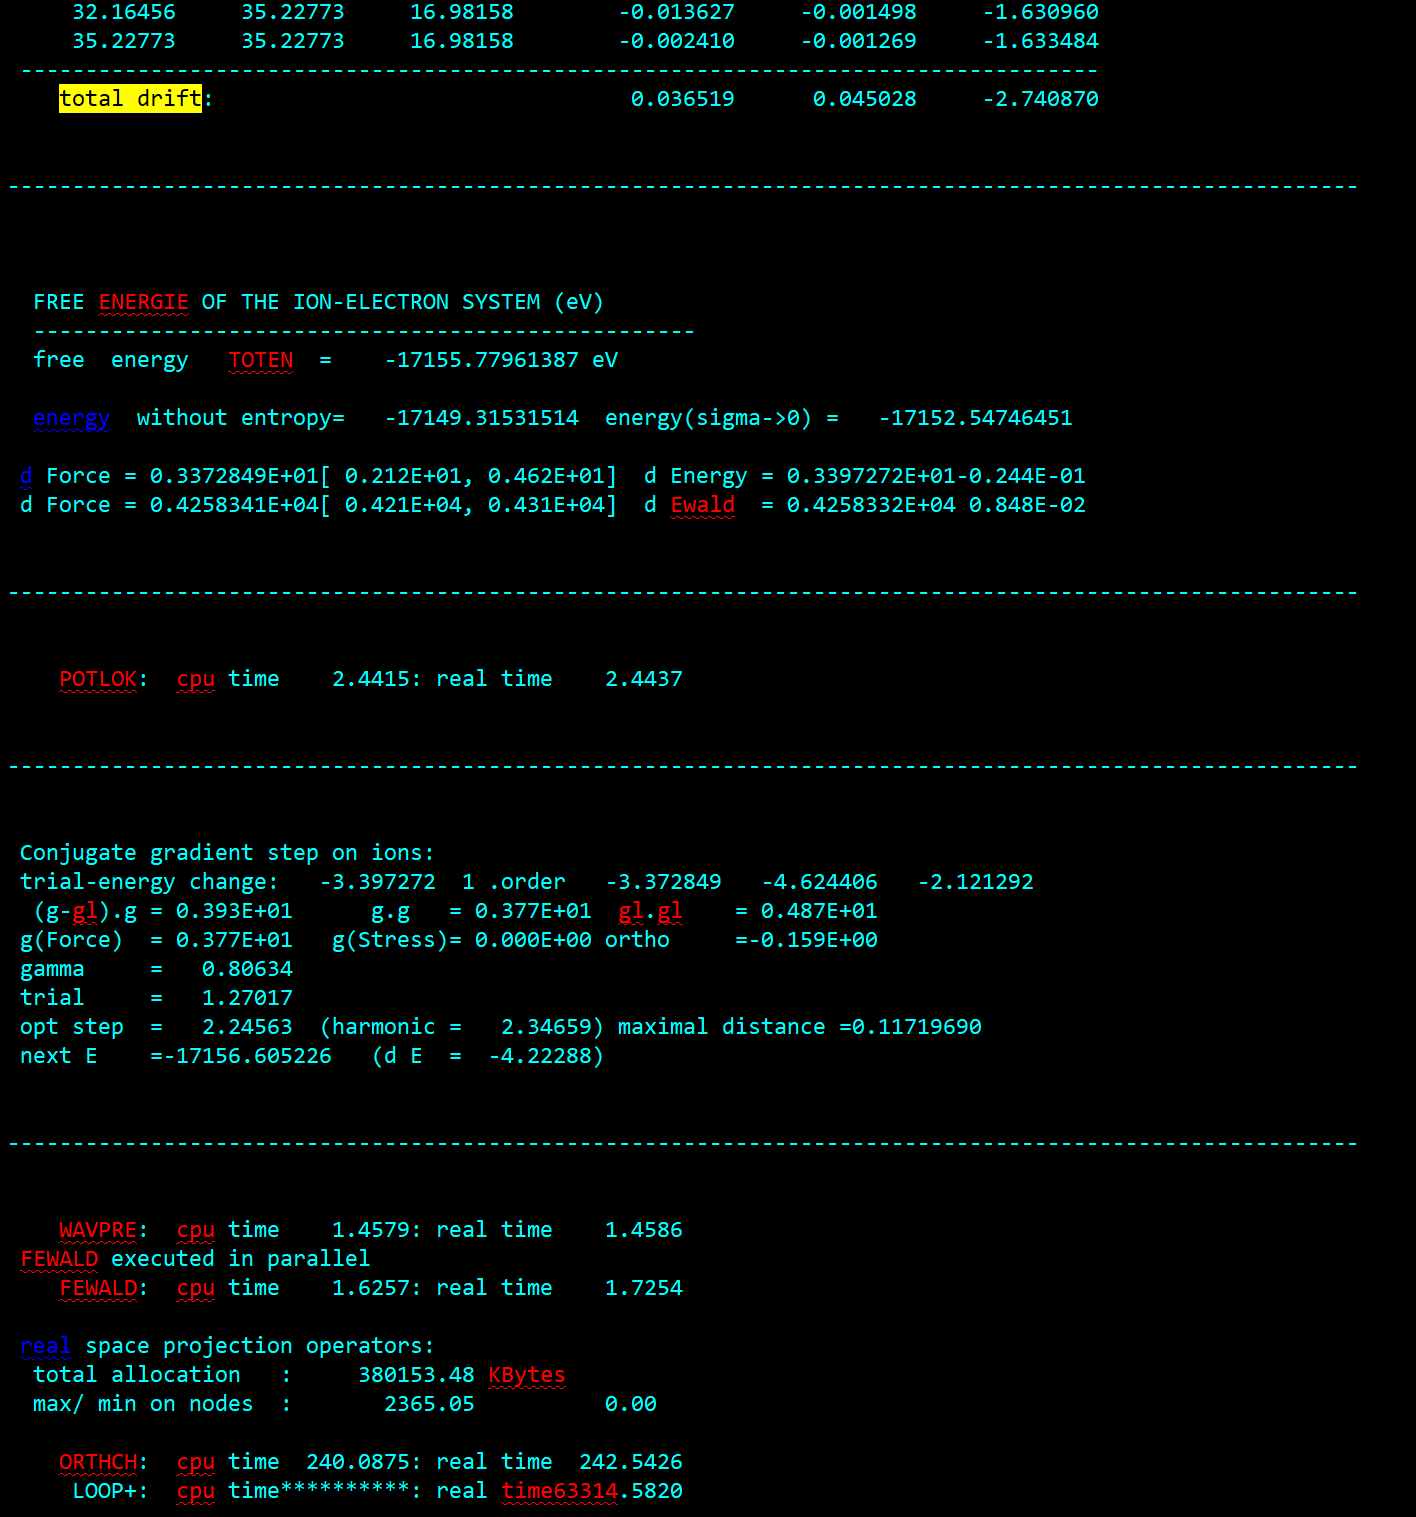
\includegraphics[height=2.15in,width=1.90in,viewport=0 0 1346 1517,clip]{Figures/VASP_huge_USTB-CFeTi_OUTCAR-1.png}
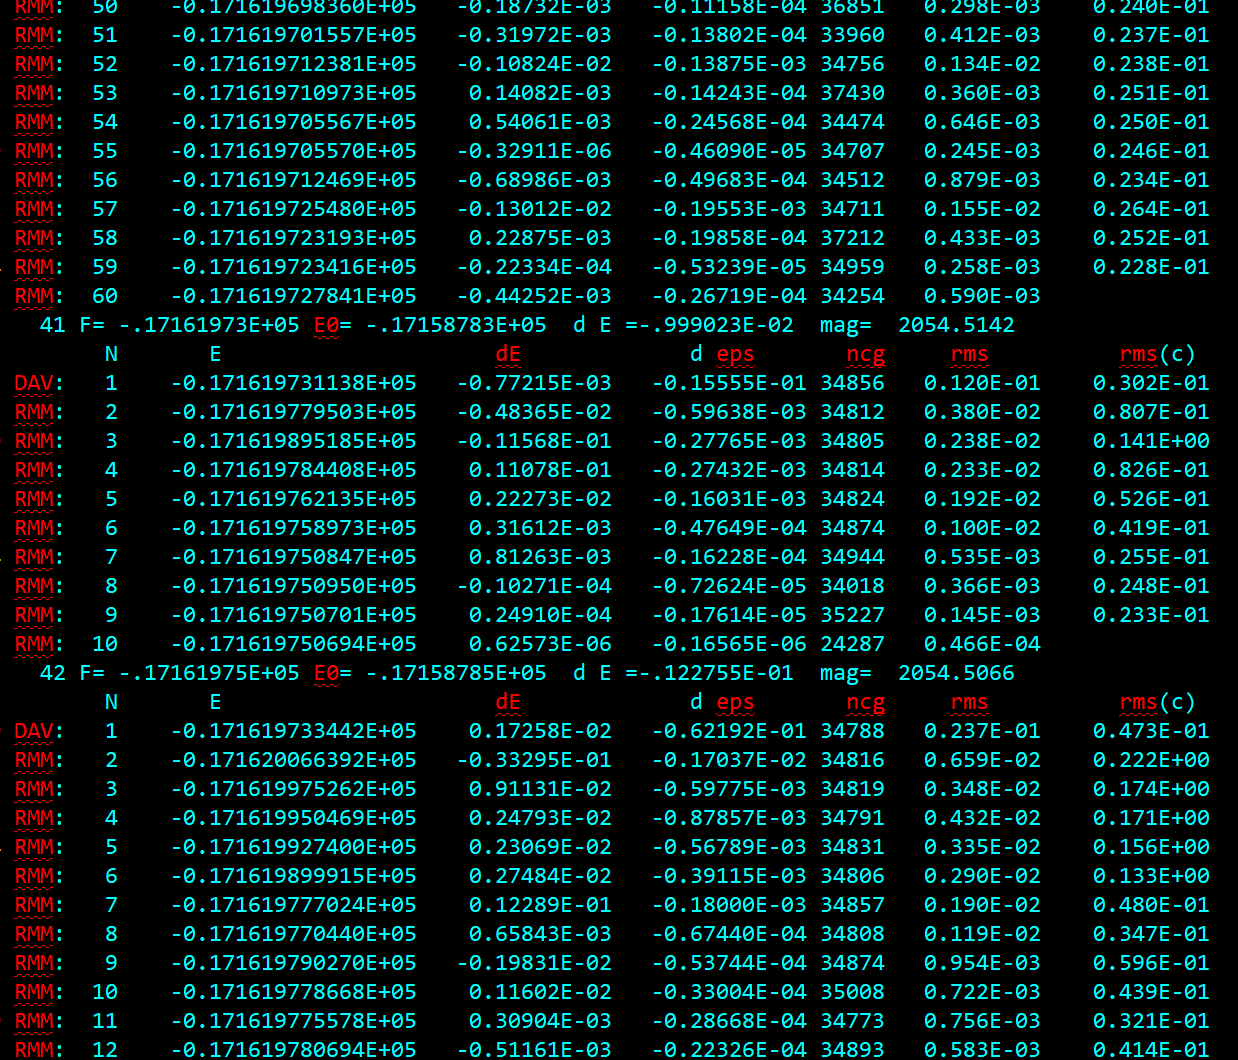
\includegraphics[height=1.05in,width=3.60in,viewport=0 150 1238 500,clip]{Figures/VASP_huge_USTB-CFeTi_OSZICAR.png}
%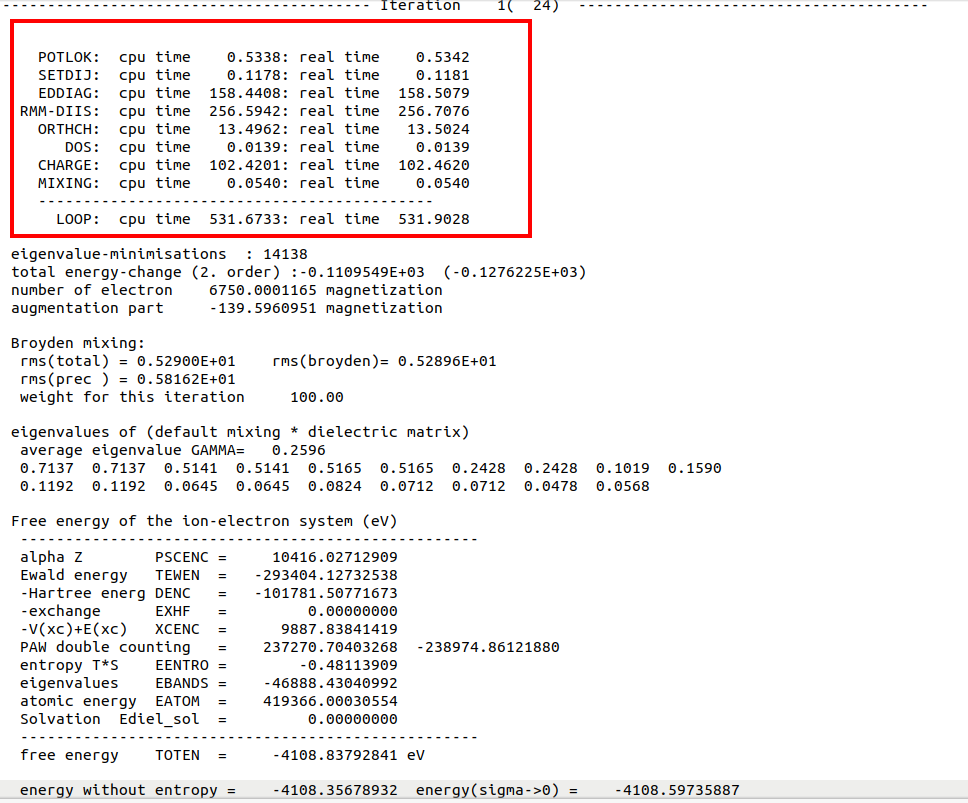
\includegraphics[height=1.35in,width=2.90in,viewport=0 560 568 803,clip]{Figures/VASP_huge_Iteration-1_24-2.png}
%\caption{\tiny \textrm{千原子合金模型($\vec k$点:~\textcolor{red}{$2\times2\times2$} vs~\textcolor{red}{$1\times1\times1$}).}}%(与文献\cite{EPJB33-47_2003}图1对比)
\label{VASP_Model-2}
\end{figure} 
\end{frame}

\begin{frame}
	\frametitle{计算算例:~\textrm{PbONICH}}
\begin{figure}[h!]
\centering
\vskip -0.21in
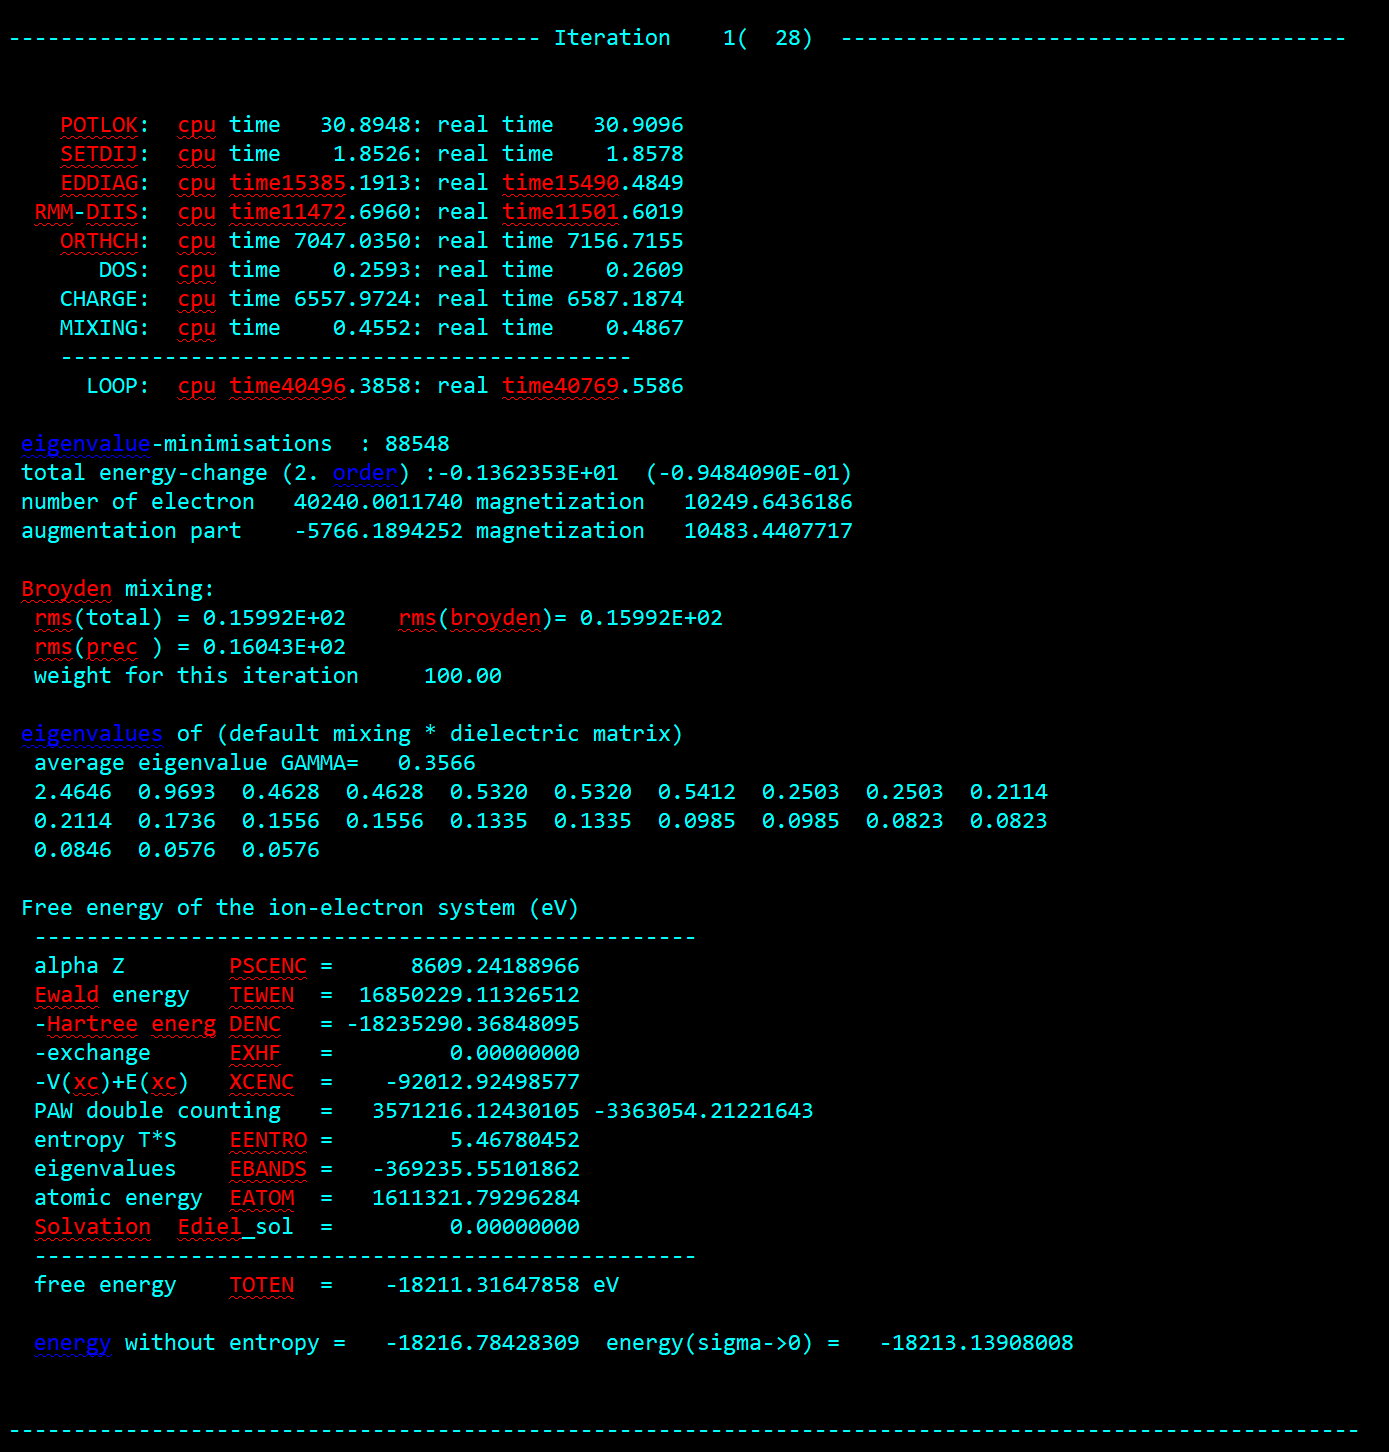
\includegraphics[height=3.05in,width=3.00in,viewport=0 0 1000 1152,clip]{Figures/VASP_huge_Ningde-PbONICH_OUTCAR.png}
%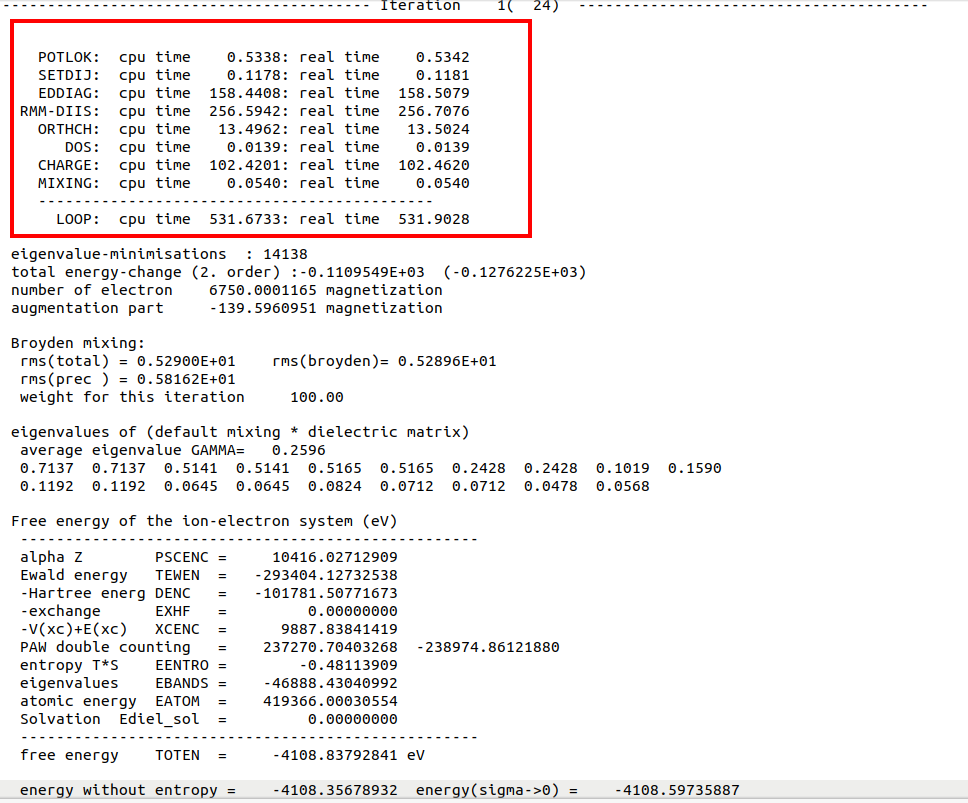
\includegraphics[height=1.35in,width=2.90in,viewport=0 560 568 803,clip]{Figures/VASP_huge_Iteration-1_24-2.png}
%\caption{\tiny \textrm{千原子合金模型($\vec k$点:~\textcolor{red}{$2\times2\times2$} vs~\textcolor{red}{$1\times1\times1$}).}}%(与文献\cite{EPJB33-47_2003}图1对比)
\label{VASP_Model-3}
\end{figure} 
\end{frame}

%\section{主要问题}
\frame
{
	\frametitle{软件价值与评估}
\textrm{VASP}支持的\textcolor{red}{$10^3$-$10^4$原子量级}模型\\
\underline{潜在的应用需求}
\begin{itemize}
		\setlength{\itemsep}{10pt}
		\item 	对机器学习势完成的分子动力学计算的实际检验:\\
			{\fontsize{7.2pt}{5.2pt}\selectfont{是否可以彻底摆脱对第一原理大规模计算的约束}}
		\item 电池材料、高熵合金的微观性质高精度计算:\\
			{\fontsize{7.2pt}{5.2pt}\selectfont{高精度的应用级模拟}}
		\item 结构材料微观缺陷的高精度模拟:\\
			{\fontsize{7.2pt}{5.2pt}\selectfont{高精度的材料可观测实验组数据对照}}
	\end{itemize}
	\vskip 5pt
	\textcolor{red}{当前算例与测试目标}:~
	\begin{itemize}
		\item 当前\textrm{VASP}支持原子规模的技术方案\underline{可靠性检验}
		\item 调研用户对$10^3$原子量级模型的\underline{计算效率预期}
	\end{itemize}
}

